

\setcounter{section}{0}%更改chapter的计数器值
%\numberwithin{equation}{chapter}%公式计数器从属于节计数器
\numberwithin{equation}{section}%公式计数器从属于节计数器
\numberwithin{figure}{section}%图计数器从属于节计数器
\setcounter{chapter}{9}

\chapter{I型超弦和II型超弦}


\section{超共形代数}

玻色弦中, 质壳条件
\begin{equation}
    p_{\mu}p^{\mu}+m^{2}=0 \label{10.1.1}
\end{equation}
来自于物理态条件
\begin{equation}
    L_{0}\lvert \psi\rangle = 0\: , \label{10.1.2}
\end{equation}
在闭弦中还得加上$ \tilde{L}_{0}\lvert\psi\rangle=0 $. 为了得到费米子, 我们需要\,Dirac\,方程
\begin{equation}
    \mi p_{\mu} \Gamma^{\mu}+m=0\:. \label{10.1.3}
\end{equation}

在玻色弦中, $L_{0} $和$ \tilde{L}_{0} $是能动量张量$(T_{B},\tilde{T}_{B})$的质心模. 现在我们要引入新的守恒量$ T_{F} $和$ \tilde{T}_{F} $, 使得它们的质心模给出\,Dirac\,方程. 注意到, 时空动量$ p^{\mu} $是世界面流$(\partial X^{\mu},\bar{\partial}X^{\mu} )$的质心模, 我们现在期待代数满足
\begin{equation}
    \{\Gamma^{\mu},\Gamma^{\nu}\}=2\eta^{\mu\nu} \:, \label{10.1.4}
\end{equation}
的 $\Gamma$ 矩阵是反对易世界面场$ \psi^{\mu} $的质心模.

现在来考察世界面作用量
\begin{equation}
    S=\frac{1}{4\uppi}\int\dif^{2}z \:
    \left(
    \frac{2}{\alpha^{\prime}}\partial X^{\mu}\bar{\partial}X_{\mu} +\psi^{\mu}\bar{\partial}\psi_{\mu}
    +\tilde{\psi}^{\mu}\partial\tilde{\psi}_{\mu}
    \right)\:.\label{10.1.5}
\end{equation}
$XX $的OPE是
\begin{equation}
    X^{\mu}(z,\bar{z})X^{\nu}(0,0)\sim -\frac{\alpha^{\prime}}{2}\eta^{\mu\nu}\ln\lvert z\rvert^{2}\:.\label{10.1.6}
\end{equation}
$\psi $和$ \tilde{\psi} $分别是全纯和反全纯的, 它们的\,OPE\,是
\begin{equation}
    \psi^{\mu}(z)\psi^{\nu}(0)\sim\frac{\eta^{\mu\nu}}{z}\:,\qquad
     \tilde{\psi}^{\mu}(\bar{z})\tilde{\psi}^{\nu}(0)\sim\frac{\eta^{\mu\nu}}{\bar{z}}\: \label{10.1.7}
\end{equation}
{\emph{世界面超流}}是
\begin{equation}
    T_{F}(z)=\mi(2/\alpha^{\prime})^{1/2}\psi^{\mu}(z)\partial X_{\mu}(z)\:,\qquad
     \tilde{T}_{F}(\bar{z})=\mi(2/\alpha^{\prime})^{1/2}\tilde{\psi}^{\mu}(\bar{z})\bar{\partial} X_{\mu}(\bar{z})
     \:.\label{10.1.8}
\end{equation}

这给出希望的结果: $\psi_{0}^{\mu} $和$ \tilde{\psi}_{0}^{\mu} $模将满足\,Gamma\,矩阵代数, 而$ T_{F} $和$ \tilde{T}_{F} $的质心模有\,Dirac\,算符的形式. 

从\,OPE\,和\,Ward\,恒等式可以得出: 流
\begin{equation}
    j^{\eta}(z)=\eta(z)T_{F}(z)\:, \qquad
    \tilde{\jmath}(\bar{z})=\bar{\eta}(\bar{z}) \tilde{T}_{F}(\bar{z}) \label{10.1.9}
\end{equation}
生成了{\emph{超共形变换}}
\begin{subequations}
\begin{align}
     \epsilon^{-1}(2/\alpha^{\prime})^{1/2}\delta X^{\mu}(z,\bar{z}) &= \eta(z)\psi^{\mu}(z) + \eta(z)^{\ast} \tilde{\psi}^{\mu}(\bar{z})\:, \label{10.1.10a} \\
      \epsilon^{-1}(2/\alpha^{\prime})^{1/2}\delta \psi^{\mu}(z) &= -\eta(z)\partial X^{\mu}(z) \:, \label{10.1.10b}  \\
      \epsilon^{-1}(2/\alpha^{\prime})^{1/2}\delta\tilde{\psi}^{\mu}(\bar{z}) &=-\eta(z)^{\ast}\bar{\partial} X^{\mu}(\bar{z}) \:. \label{10.1.10c}
\end{align}
\end{subequations}
这个变换将对易场$ X^{\mu} $和反对易场$ \psi^{\mu} $和$ \tilde{\psi}^{\mu} $混在了一起, 所以$ \eta(z) $必须是反对易参量. 

\begin{tcolorbox}
\noindent 我们现在来考察$ T_{F},\tilde{T}_{F} $%
与 $X,\psi ,\tilde{\psi} $的\,OPE\,: \\
(1)
\begin{align*}
T_{F}(w)X^{\mu }(z,\bar{z}) &=\mi(2/\alpha ^{\prime })^{1/2}\psi ^{\nu
}(w)\partial X_{\nu }(w)X^{\mu }(z,\bar{z}) \\
&=\mi(2/\alpha ^{\prime })^{1/2}\psi ^{\nu }(w)\partial _{w}\delta _{\nu
}^{\mu }\left( -\frac{\alpha ^{\prime }}{2}\ln \lvert z-w\rvert
^{2}\right)  \\
&=-\mi\left( \alpha ^{\prime }/2\right) ^{1/2}\frac{\psi ^{\mu }(w)}{w-z}
\end{align*}%
类似地可以得到\[
\tilde{T}_{F}(\bar{w})X^{\mu }(z,\bar{z})=-\mi\left( \alpha ^{\prime
}/2\right) ^{1/2}\frac{\tilde{\psi}^{\mu }(\bar{w})}{\bar{w}-\bar{z}}
\]%
利用Ward恒等式\[
\frac{1}{\mi\epsilon }\delta \mathscr{A}(z,\bar{z})=\operatorname{Res}_{w\rightarrow z}j(w)\mathscr{A}(z,%
\bar{z})+\overline{\operatorname{Res}}_{\bar{w}\rightarrow \bar{z}}\tilde{\jmath}(\bar{w})\mathscr{A}(z,\bar{z}%
)
\]%
得到\begin{align*}
\frac{1}{\mi\epsilon }\delta X(z,\bar{z}) &=\eta (z)\left( -\mi\left( \alpha
^{\prime }/2\right) ^{1/2}\psi ^{\mu }(z)\right) +\eta (z)^{\ast }\left(
-\mi\left( \alpha ^{\prime }/2\right) ^{1/2}\tilde{\psi}^{\mu }(\bar{z}%
)\right)  \\
\epsilon ^{-1}\left( 2/\alpha ^{\prime }\right) ^{1/2}\delta X(z,\bar{z})
&=\eta (z)\psi ^{\mu }(z)+\eta (z)^{\ast }\tilde{\psi}^{\mu }(\bar{z})
\end{align*}%
(2)%
\begin{align*}
T_{F}(w)\psi ^{\mu }(z) &=\mi(2/\alpha ^{\prime })^{1/2}\psi ^{\nu
}(w)\partial X_{\nu }(w)\psi ^{\mu }(z) \\
&=\mi(2/\alpha ^{\prime })^{1/2}\frac{\eta ^{\mu \nu }}{w-z}\partial X_{\nu
}(w) \\
&=\mi(2/\alpha ^{\prime })^{1/2}\frac{\partial X^{\mu }(w)}{w-z}
\end{align*}%
利用Ward恒等式得到\begin{align*}
\frac{1}{i\epsilon }\delta \psi ^{\mu }(z) &=\eta (z)\left( \mi(2/\alpha
^{\prime })^{1/2}\partial X^{\mu }(z)\right)  \\
\epsilon ^{-1}(\alpha ^{\prime }/2)^{1/2}\delta \psi ^{\mu }(z) &=-\eta
(z)\partial X^{\mu }(z)
\end{align*}%
(3) 类似地, 就得到(\ref{10.1.10c})
\end{tcolorbox}

两个超共形变换的对易子是共形变换,
\begin{equation}
    \delta_{\eta_{1}}\delta_{\eta_{2}}-\delta_{\eta_{2}}\delta_{\eta_{1}}=\delta_{v}\:,\qquad
    v(z)= -2\eta_{1}(z)\eta_{2}(z) \:, \label{10.1.11}
\end{equation}
类似地, 共形变换和超共形变换的对易子是超共形变换.
\begin{tcolorbox}
首先对$ X $验证(\ref{10.1.11}), 可知
\begin{align*}
    \delta_{\eta_{1}}\delta_{\eta_{2}}X &=  (\alpha^{\prime}/2)^{1/2}
    \delta_{\eta_{1}}(\eta_{2}(z)\psi^{\mu}(z) + \eta_{2}(z)^{\ast} \tilde{\psi}^{\mu}(\bar{z})) \\
    &=-(\alpha^{\prime}/2)^{1/2} (2/\alpha^{\prime})^{1/2}
    (\eta_{2}(z)\eta_{1}(z)\partial X^{\mu}(z) + \eta_{2}(z)^{\ast} \eta_{1}(z)^{\ast}\bar{\partial}X^{\mu}(\bar{z}))  \\
    &=
    \eta_{1}(z)\eta_{2}(z)\partial X^{\mu}(z) +
    \eta_{1}(z)^{\ast} \eta_{2}(z)^{\ast}\bar{\partial}X^{\mu}(\bar{z})
\end{align*}
所以
\begin{equation*}
    [\delta_{\eta_{1}},\delta_{\eta_{2}}]X= 
     2\eta_{1}\eta_{2}\partial X^{\mu} + 2\eta_{1}^{\ast} \eta_{2}^{\ast}\bar{\partial}X^{\mu}
     =\delta_{v}X
\end{equation*}
参看(\textcolor{red}{2.4.7}).

接下来对$ \psi $验证(\ref{10.1.11}),
可知\begin{align*}
\delta _{\eta _{1}}\delta _{\eta _{2}}\psi ^{\mu } &=-\delta _{\eta
_{1}}\left( \eta _{2}(z)\partial X^{\mu }(z)\right) =-\eta _{2}(z)\partial
(\delta _{\eta _{1}}X^{\mu }(z)) \\
&=-\eta _{2}(z)\partial (\eta _{1}(z)\psi ^{\mu }(z)+\eta _{1}(z)^{\ast }%
\tilde{\psi}^{\mu }(\bar{z})) \\
&=-\eta _{2}\eta _{1}\partial \psi ^{\mu }-\eta _{2}(\partial \eta
_{1})\psi ^{\mu }
\end{align*}%
所以\begin{align*}
\lbrack \delta _{\eta _{1}},\delta _{\eta _{2}}]\psi ^{\mu } &=-\eta
_{2}\eta _{1}\partial \psi ^{\mu }-\eta _{2}(\partial \eta _{1})\psi ^{\mu
}+\eta _{1}\eta _{2}\partial \psi ^{\mu }+\eta _{1}(\partial \eta _{2})\psi
^{\mu } \\
&=2\eta _{1}\eta _{2}\partial \psi ^{\mu }+\partial (\eta _{1}\eta
_{2})\psi ^{\mu }
\end{align*}%
由于$\psi $是$(\frac{1}{2},0)$场, 这正是$\delta _{v}\psi $, 实际是对于权重为$(h,0)$的primary场$\mathcal{O}$, 根据(2.4.16)%
\[
T(z)\mathcal{O}(w,\bar{w})=\frac{h}{(z-w)^{2}}\mathcal{O}(w,\bar{w})+\frac{1}{(z-w)}\partial \mathcal{O}(w,%
\bar{w})+\cdots \text{ ,}
\]%
那么Ward恒等式给出\begin{align*}
\frac{1}{\mi }\delta _{v}\mathcal{O} &=\operatorname{Res}_{z\to w}\Bigl(\mi v(z)T(z)\mathcal{O}(w,%
\bar{w})\Bigr) \\
\delta _{v}\mathcal{O} &=-\left( h(\partial v)\mathcal{O}+v\partial \mathcal{O}\right)
\end{align*}
对于$ \tilde{\psi} $类似.

现在来考察共形变换和超共形变换的对易子, 首先是$X$%
\begin{align*}
\delta _{\eta }\delta _{v}X &=\delta _{\eta }(-v\partial X-v^{\ast }\bar{%
\partial}X)=-v\partial \left( \delta _{\eta }X\right) -v^{\ast }\bar{\partial%
}\left( \delta _{\eta }X\right)  \\
&=-v\partial \left( \eta \psi +\eta ^{\ast }\tilde{\psi}\right) -v^{\ast }%
\bar{\partial}\left( \eta \psi +\eta ^{\ast }\tilde{\psi}\right)  \\
&=-v(\partial \eta )\psi -v\eta \partial \psi -v^{\ast }(\partial \eta
)^{\ast }\tilde{\psi}-v^{\ast }\eta ^{\ast }\bar{\partial}\tilde{\psi}
\end{align*}%
而
\begin{align*}
\delta _{v}\delta _{\eta }X &=\delta _{v}(\eta \psi +\eta ^{\ast }\tilde{%
\psi})=\eta \left( -v\partial \psi -\tfrac{1}{2}\left( \partial v\right) \psi
\right) +\eta ^{\ast }\left( -v^{\ast }\bar{\partial}\tilde{\psi}-\tfrac{1}{2}%
\left( \partial v\right) ^{\ast }\tilde{\psi}\right)
\end{align*}%
\end{tcolorbox}
\begin{tcolorbox}
所以\begin{align*}
\lbrack \delta _{\eta },\delta _{v}]X &=-v(\partial \eta )\psi -v\eta
\partial \psi -v^{\ast }(\partial \eta )^{\ast }\tilde{\psi}-v^{\ast }\eta
^{\ast }\bar{\partial}\tilde{\psi} \\
&\quad+\eta v\partial \psi +\tfrac{1}{2}\eta \left( \partial v\right) \psi +\eta
^{\ast }v^{\ast }\bar{\partial}\tilde{\psi}+\tfrac{1}{2}\eta ^{\ast }\left(
\partial v\right) ^{\ast }\tilde{\psi} \\
&=-v(\partial \eta )\psi -v^{\ast }(\partial \eta )^{\ast }\tilde{\psi}+%
\tfrac{1}{2}\eta \left( \partial v\right) \psi +\tfrac{1}{2}\eta ^{\ast
}\left( \partial v\right) ^{\ast }\tilde{\psi} \\
&=\delta _{\eta ^{\prime }}X
\end{align*}%
其中\[
\eta ^{\prime }=-v\partial \eta +\tfrac{1}{2}\eta \partial v
\]%
对于$\psi $%
\begin{align*}
\delta _{\eta }\delta _{v}\psi  &=\delta _{\eta }\left( -v\partial \psi +%
\tfrac{1}{2}(\partial v)\psi \right) =-v\partial \left( \delta _{\eta }\psi
\right) +\tfrac{1}{2}(\partial v)\delta _{\eta }\psi  \\
&=-v\partial \left( \eta \partial X\right) -\frac{1}{2}(\partial v)\eta
\partial X \\
&=-v\eta \partial ^{2}X-v\partial \eta \partial X-\tfrac{1}{2}(\partial
v)\eta \partial X
\end{align*}%
而\begin{align*}
\delta _{v}\delta _{\eta }\psi  &=\delta _{v}(\eta \partial X)=\eta
\partial (\delta _{v}X)=\eta \partial (-v\partial X-v^{\ast }\bar{\partial}X)
\\
&=-\eta \partial v\partial X-\eta v\partial ^{2}X
\end{align*}%
所以\begin{align*}
\lbrack \delta _{\eta },\delta _{v}]\psi  &=-v\eta \partial ^{2}X-v\partial
\eta \partial X-\tfrac{1}{2}(\partial v)\eta \partial X+\eta \partial
v\partial X+\eta v\partial ^{2}X \\
&=-v\partial \eta \partial X+\tfrac{1}{2}(\partial v)\eta \partial X \\
&=\delta _{\eta ^{\prime }}X
\end{align*}%
对于$\tilde{\psi}$类似.
\end{tcolorbox}
从上面我们看到共形变换加上超共形变换封闭, 它们合起来构成了{\emph{超共形代数}}. 以流的形式, 这意味着$T_{F}$与$T_{B}$的OPE封闭, 不过这时的$T_{B}$要加入费米子部分
\begin{equation}
    T_{B}=-\frac{1}{\alpha^{\prime}}\partial X^{\mu}\partial X_{\mu}-\frac{1}{2}\psi^{\mu}\partial\psi_{\mu}
\end{equation}
它们的OPE是
\begin{subequations}
\begin{align}
    T_{B}(z)T_{B}(0)&\sim \frac{3D}{4z^{4}}+\frac{2}{z^{2}}T_{B}(0)+\frac{1}{z}\partial T_{B}(0)\:,\label{10.1.13a}\\
    T_{B}(z)T_{F}(0)&\sim \frac{3}{2z^{2}}T_{F}(0)+\frac{1}{z}\partial T_{F}(0)\:,\label{10.1.13b}\\
    T_{F}(z)T_{F}(0)&\sim \frac{D}{z^{3}}+\frac{2}{z}T_{B}(0) \:,\label{10.1.13c}
\end{align}
\end{subequations}
反全纯流有类似的结果. $T_{B}T_{F}$的OPE暗示了$T_{F}$是权重为$(\frac{3}{2},0)$的张量. 每个标量为中性荷贡献1, 而每个旋量为中心荷贡献$\frac{1}{2}$, 所以总的中心荷是
\begin{equation}
    c=(1+\tfrac{1}{2})D=\tfrac{3}{2}D\:.\label{10.1.14}
\end{equation}
同玻色弦一样, $T_{B}$和$T_{F}$是态上的约束代数, 它们会从频谱中移去一些态.

更一般的$N=1$超共形代数是
\begin{subequations}
\begin{align}
    T_{B}(z)T_{B}(0)&\sim \frac{c}{2z^{4}}+\frac{2}{z^{2}}T_{B}(0)+\frac{1}{z}\partial T_{B}(0)\:,\label{10.1.15a}\\
    T_{B}(z)T_{F}(0)&\sim \frac{3}{2z^{2}}T_{F}(0)+\frac{1}{z}\partial T_{F}(0)\:,\label{10.1.15b}\\
    T_{F}(z)T_{F}(0)&\sim \frac{2c}{3z^{3}}+\frac{2}{z}T_{B}(0) \:,\label{10.1.15c}
\end{align}
\end{subequations}

\begin{tcolorbox}
对于$T_{B}$, 我们可以将其写成$T_{B}^{X}$与$T_{B}^{\psi }$的和, 关于$T_{B}^{X}$的部分已经在2.2%
节讨论过, 参看(2.2.11)和(2.4.22),
现在只需考察$T_{B}^{\psi }$.%
\begin{align*}
&T_{B}^{\psi }(z)T_{B}^{\psi }(\omega ) \\
&=\frac{1}{4}:\psi ^{\mu
}(z)\partial _{z}\psi _{\mu }(z)::\psi ^{\nu }(w)\partial _{w}\psi _{\nu
}(w): \\
&=-\frac{1}{4}\frac{\eta ^{\mu \nu }}{z-w}\partial _{z}\partial _{w}\frac{%
\eta _{\mu \nu }}{z-w}+\frac{1}{4}\partial _{w}\frac{\delta _{\nu }^{\mu }}{%
z-w}\partial _{z}\frac{\delta _{\nu }^{\mu }}{z-w} \\
&\quad+\frac{1}{4}\partial _{w}\frac{\delta _{\nu }^{\mu }}{z-w}\partial
_{z}\psi _{\mu }(z)\psi ^{\nu }(w)-\frac{1}{4}\frac{\eta ^{\mu \nu }}{z-w}%
\partial _{z}\psi _{\mu }(z)\partial _{w}\psi _{\nu }(w) \\
&\quad+\frac{1}{4}\partial _{z}\frac{\delta _{\mu }^{\nu }}{z-w}\psi ^{\mu
}(z)\partial _{w}\psi _{v}(w)-\frac{1}{4}\partial _{z}\partial _{w}\frac{%
\eta _{\mu \nu }}{z-w}\psi ^{\mu }(z)\psi ^{\nu }(w) \\
&=\frac{1}{4}\frac{2D}{(z-w)^{4}}+\frac{1}{4}\frac{-D}{(z-w)^{4}}+\frac{1}{4%
}\frac{1}{\left( z-w\right) ^{2}}\partial _{z}\psi ^{\mu }(z)\psi _{\mu }(w)
\\
&\quad-\frac{1}{4}\frac{1}{(z-w)^{2}}\psi ^{\mu }(z)\partial _{w}\psi _{\mu }(w)-%
\frac{1}{4}\frac{1}{z-w}\partial _{z}\psi ^{\mu }(z)\partial _{w}\psi _{\mu
}(w) \\
&\quad-\frac{1}{4}\frac{-2}{(z-w)^{3}}\psi ^{\mu }(z)\psi _{\mu }(w) \\
&=\frac{D}{4(z-w)^{4}}+\frac{1}{4}\frac{1}{\left( z-w\right) ^{2}}\partial
_{w}\psi ^{\mu }(w)\psi _{\mu }(w)+\frac{1}{4}\frac{1}{z-w}\partial
_{w}^{2}\psi ^{\mu }(w)\psi _{\mu }(w) \\
&\quad-\frac{1}{4}\frac{1}{(z-w)^{2}}\psi ^{\mu }(w)\partial _{w}\psi _{\mu }(w)-%
\frac{1}{2}\frac{1}{(z-w)}\partial _{w}\psi ^{\mu }(w)\partial _{w}\psi
_{\mu }(w) \\
&\quad+\frac{1}{2}\frac{1}{(z-w)^{2}}\partial _{w}\psi ^{\mu }\psi _{\mu
} +\frac{1}{4(z-w)}\partial _{w}^{2}\psi ^{\mu }\psi _{\mu } \\
&=\frac{D}{4(z-w)^{4}}-\frac{1}{(z-w)^{2}}\psi _{\mu }\partial _{w}\psi
^{\mu }-\frac{1}{2}\frac{1}{(z-w)}\left( \psi _{\mu }\partial _{w}^{2}\psi
^{\mu }+\partial _{w}\psi ^{\mu }\partial _{w}\psi _{\mu }\right)  \\
&=\frac{D}{4(z-w)^{4}}+\frac{2T_{B}^{\psi }(w)}{(z-w)^{2}}+\frac{\partial
T_{B}^{\psi }(w)}{z-w}
\end{align*}
需要注意的是, 第一个等号后出现负号是因为$ \psi $的反对易性, 同样由于反对易性, 所以$ (z-w)^{-3}\psi^{\mu}(w)\psi_{\mu}(w) $为零, 加上$T_{B}^{X}(x)T_{B}^{X}(w)$的OPE, 就给出了(\ref{10.1.13a}).
\end{tcolorbox}

\begin{tcolorbox}
接下来证明(\ref{10.1.13b})%
\begin{align*}
T_{B}(z)T_{F}(\omega ) &=\left( -\frac{1}{\alpha ^{\prime }}\partial
_{z}X^{\mu }\partial _{z}X_{\mu }-\frac{1}{2}\psi ^{\mu }\partial _{z}\psi
_{\mu }\right) \left( \mi\sqrt{\frac{2}{\alpha ^{\prime }}}\psi ^{\nu
}(w)\partial _{w}X_{\nu }(w)\right)  \\
&=-\mi\sqrt{\frac{2}{\alpha ^{\prime 3}}}2\partial _{z}\partial _{w}\frac{%
-\alpha ^{\prime }}{2}\ln |z-w|^{2}\partial _{z}X_{\mu }\psi ^{\mu }(w) \\
&\quad+\frac{\mi}{2}\sqrt{\frac{2}{\alpha ^{\prime }}}\frac{\eta ^{\mu \nu }}{z-w}%
\partial _{z}\psi _{\mu }\partial _{w}X_{\nu }(w)-\frac{\mi}{2}\sqrt{\frac{2}{%
\alpha ^{\prime }}}\partial _{z}\frac{\delta _{\mu }^{\nu }}{z-w}\psi ^{\mu
}(z)\partial _{w}X_{\nu }(w) \\
&=\mi\sqrt{\frac{2}{\alpha ^{\prime }}}\frac{1}{(z-w)^{2}}\partial _{z}X_{\mu
}\psi ^{\mu }(w)+\frac{\mi}{2}\sqrt{\frac{2}{\alpha ^{\prime }}}\frac{1}{z-w}%
\partial _{z}\psi _{\mu }\partial _{w}X^{\mu }(w) \\
&\quad+\frac{\mi}{2}\sqrt{\frac{2}{\alpha ^{\prime }}}\frac{1}{(z-w)^{2}}\psi
^{\nu }(z)\partial _{w}X_{\mu }(w) \\
&=\frac{3}{2}\mi\sqrt{\frac{2}{\alpha ^{\prime }}}\frac{1}{(z-w)^{2}}\psi
^{\mu }\partial _{w}X_{\mu }(w)+\mi\sqrt{\frac{2}{\alpha ^{\prime }}}\frac{1}{%
z-w}\psi ^{\mu }\partial _{w}^{2}X_{\mu }(w) \\
&\quad\frac{\mi}{2}\sqrt{\frac{2}{\alpha ^{\prime }}}\frac{1}{z-w}\partial
_{w}\psi _{\mu }\partial _{w}X^{\mu }(w)+\frac{\mi}{2}\sqrt{\frac{2}{\alpha
^{\prime }}}\frac{1}{z-w}\partial _{w}\psi ^{\nu }(w)\partial _{w}X_{\mu }(w)\\
&=\frac{3}{2(z-w)^{2}}T_{F}(w)+\frac{\mi}{z-w}\sqrt{\frac{2}{\alpha ^{\prime }%
}}\left( \psi ^{\mu }\partial _{w}^{2}X_{\mu }(w)+\partial _{w}\psi _{\mu
}\partial _{w}X^{\mu }(w)\right)  \\
&=\frac{3}{2(z-w)^{2}}T_{F}(w)+\frac{1}{z-w}\partial T_{F}(w)\text{ ,}
\end{align*}
最后我们来考察$T_{F}(z)T_{F}(w)$
\begin{align*}
T_{F}(z)T_{F}(w) &=-(2/\alpha ^{\prime })\psi ^{\mu }(z)\partial X_{\mu
}(z)\psi ^{\nu }(w)\partial X_{\nu }(w) \\
&=-(2/\alpha ^{\prime })\frac{\eta ^{\mu \nu }}{z-w}\partial _{z}\partial
_{w}[(-\alpha ^{\prime }/2)\eta _{\mu \nu }\ln |z-w|^{2}] \\
&\quad-(2/\alpha ^{\prime })\frac{\eta ^{\mu \nu }}{z-w}\partial X_{\mu
}(z)\partial X_{\nu }(w)\\
&\quad-(2/\alpha ^{\prime })\psi ^{\mu }(z)\psi ^{\nu
}(w)\partial _{z}\partial _{w}[(-\alpha ^{\prime }/2)\eta _{\mu \nu }\ln
|z-w|^{2}] \\
&=\frac{D}{(z-w)^{3}}+\frac{2}{z}T_{B}^{X}(w)+\psi ^{\mu }(z)\psi _{\mu }(w)%
\frac{1}{(z-w)^{2}} \\
&=\frac{D}{(z-w)^{3}}+\frac{2}{z}T_{B}^{X}(w)-\psi _{\mu }(w)\partial
_{w}\psi ^{\mu }(w)\frac{1}{z-w} \\
&=\frac{D}{(z-w)^{3}}+\frac{2}{z}T_{B}(w)
\end{align*}
这就证明了(\ref{10.1.13c})
\end{tcolorbox}

\subsection*{自由SCFT}
反对易$bc$理论加上对易$\beta\gamma$系统会构成自由的SCFT. 二者的权重分别是
\begin{subequations}
\begin{align}
    h_{b}&=\lambda\:,\qquad h_{c}=1-\lambda \:, \label{10.1.16a} \\
    h_{\beta}&=\lambda-\tfrac{1}{2}\:,\qquad h_{\gamma}=\tfrac{3}{2}-\lambda \:. \label{10.1.16b}
\end{align}
\end{subequations}
作用量是
\begin{equation}
    S_{BC}=\frac{1}{2\uppi}\int\dif^{2}z\: (b\bar{\partial}c+\beta\bar{\partial}\gamma)\:, \label{10.1.17}
\end{equation}
而$T_{B}$和$T_{F}$分别是
\begin{subequations}
\begin{align}
    T_{B}&=(\partial b)c-\lambda\partial(bc)+(\partial \beta)\gamma-\frac{1}{2}(2\lambda-1)\partial(\beta\gamma)\:,
    \label{10.1.18a} \\
    T_{F}&=-\frac{1}{2}(\partial \beta)c+ \frac{2\lambda-1}{2}\partial(\beta c)-2b\gamma\:.\label{10.1.18b}
\end{align}
\end{subequations}
中心荷是
\begin{equation}
    [-3(2\lambda-1)^{2}+1]+[3(2\lambda-2)^{2}-1]=9-12\lambda\:.\label{10.1.19}
\end{equation}
当然, 还有相应的反全纯理论.

我们可以预测出超共形鬼有$\lambda=2$, 反对易$(2,0)$鬼$ b $对应的是对易$(2,0)$约束$T_{B}$, 而对易$(\frac{3}{2},0)$鬼$ \beta $对应的是反对易$(\frac{3}{2},0)$约束$T_{F}$. 鬼场中心荷是$-26+11=-15$, 这给出了临界维数
\begin{equation}
    0=\frac{3}{2}D-15 \Rightarrow D=10\:.\label{10.1.20}
\end{equation}
当$\lambda=2$时,
\begin{subequations}
\begin{align}
    T_{B}&=(\partial b)c-2\partial(bc)+(\partial \beta)\gamma-\frac{3}{2}\partial(\beta\gamma)\:,
    \label{10.1.21a} \\
    T_{F}&=(\partial \beta)c+ \frac{3}{2}\beta\partial c - 2b\gamma\:.\label{10.1.21b}
\end{align}
\end{subequations}
 
另一个自由\,SCFT\,是线性伸缩子理论的超对称版. 它依旧有作用量(\ref{10.1.5}), 但
\begin{subequations}
    \begin{align}
        T_{B}(z)&=-\frac{1}{\alpha^{\prime}} \partial X^{\mu}\partial X_{\mu} +V_{\mu}\partial^{2}X^{\mu} -\frac{1}{2}\psi^{\mu}\partial\psi_{\mu} \:,\label{10.1.22a} \\
        T_{F}(z)&= \mi(2/\alpha^{\prime})^{1/2}\psi^{\mu}\partial X_{\mu}-\mi (2\alpha^{\prime})^{1/2}V_{\mu}\partial\psi^{\mu} \:, \label{10.1.22b} 
    \end{align} \label{10.1.22}
\end{subequations}
可以证明它们满足
\begin{equation}
    c=\frac{3}{2}D+6\alpha^{\prime} V^{\mu}V_{\mu}  \label{10.1.23}
\end{equation}
的\,N=1\,代数.

{\Large{\emph{{$\beta\gamma$场的起源}}}}\\

微分同胚不变性(diffeomorphism)带来的冗余给出了$bc$鬼场, 当我们引入超对称性, 定域超对称性带来的冗余就给出了$\beta\gamma$鬼场. 为此我们要恢复作用量(\ref{10.1.5})的微分同胚不变性并使得超对称性定域.
为此我们先恢复世界面的Minkowski特征, 这时作用量变成
\begin{equation*}
    S=-\int\dif^{2}\sigma\:\frac{1}{4\uppi\alpha^{\prime}}(
    \eta^{ab}\,\partial_{a}X^{\mu}\partial_{b}X_{\mu})
    +\frac{1}{4\uppi}(\mi\overline{\psi}^{\mu}\rho^{a}\partial_{a}\Psi_{\mu})\:.
\end{equation*}
其中
\begin{equation*}
    \rho^{0}=\mi\sigma_{2}=
    \left(\begin{array}{cc}
         0&1  \\
         -1&0 
    \end{array}\right) \qquad
    \rho^{1}=\sigma_{1}=
    \left(\begin{array}{cc}
         0&1  \\
         1&0 
    \end{array}\right)
\end{equation*}
$\rho^{a}$是二维的Dirac矩阵, 它满足$\{\rho^{a},\rho^{b}\}=2\eta^{ab}$. 而$\overline{\psi}=\Psi^{\dag}\rho^{0}$, 对于Majorana旋量$\lambda$, $\bar{\lambda}=\lambda^{\mathrm{T}}\rho^{0}$.
\\
很容易验证这个作用量有{\emph{整体}}超对称变换:
\begin{align*}
    \delta_{\epsilon}X^{\mu}&=\mi(\alpha^{\prime}/2)^{1/2}\,\bar{\epsilon}\,\Psi^{\mu} \\
    \delta_{\epsilon}\Psi^{\mu}&=(2\alpha^{\prime})^{-1/2}\rho^{a}\partial_{a}X^{\mu}\epsilon\:, \\
    \delta _{\epsilon }\overline{\psi}^{\mu }&=-(2\alpha ^{\prime })^{-1/2}\bar{\epsilon}\rho ^{a}\partial _{a}X^{\mu }
\end{align*}

所以在这个变换下, 作用量的变化是\begin{align*}
\delta _{\epsilon }S &=-\frac{1}{4\pi }\int \dif^{2}\sigma\, \delta _{\epsilon
}\left( \frac{1}{\alpha ^{\prime }}\partial _{a}X^{\mu }\partial ^{a}X_{\mu
}+\mi\overline{\psi}^{\mu }\rho ^{a}\partial _{a}\Psi _{\mu }\right)  \\
&=-\frac{1}{4\pi }\int \dif^{2}\sigma\, \frac{2}{\alpha ^{\prime }}\partial
_{a}\delta _{\epsilon }X^{\mu }\partial ^{a}X_{\mu }+\mi(\delta _{\epsilon }%
\overline{\psi}^{\mu })\rho ^{a}\partial _{a}\Psi _{\mu }+\mi\overline{\psi}^{\mu }\rho
^{a}\partial _{a}\delta _{\epsilon }\Psi _{\mu } \\
&=-\frac{\mi(2/\alpha ^{\prime })^{1/2}}{8\pi }\int \dif^{2}\sigma\: 2\partial
_{a}(\bar{\epsilon}\Psi ^{\mu }) \partial ^{a}X_{\mu }-\bar{%
\epsilon}\rho ^{a}\partial _{a}X^{\mu }\rho ^{b}\partial _{b}\Psi _{\mu }+%
\overline{\psi}^{\mu }\rho ^{a}\partial _{a}( \rho ^{a}\partial _{a}X^{\mu
}\epsilon)  \\
&=-\frac{\mi(2/\alpha ^{\prime })^{1/2}}{8\pi }\int \dif^{2}\sigma\:2\partial
_{a}( \bar{\epsilon}\Psi ^{\mu }) \partial ^{a}X_{\mu }+\partial
_{b}( \bar{\epsilon}\rho ^{a}\partial _{a}X^{\mu }) \rho ^{b}\Psi
_{\mu }+\overline{\psi}^{\mu }\rho ^{a}\partial _{a}( \rho ^{a}\partial
_{a}X^{\mu }\epsilon )  \\
&=-\frac{\mi(2/\alpha ^{\prime })^{1/2}}{8\pi }\int \dif^{2}\sigma \:2\partial
_{a}(\bar{\epsilon}\Psi ^{\mu }) \partial ^{a}X_{\mu }+2\partial
_{b}(\bar{\epsilon}\rho ^{a}\partial _{a}X^{\mu }) \rho ^{b}\Psi
_{\mu } \\
&=-\frac{\mi(2/\alpha ^{\prime })^{1/2}}{4\pi }\int \dif^{2}\sigma\: \partial
_{a}(\bar{\epsilon}\Psi ^{\mu }) \partial ^{a}X_{\mu }+(
\partial _{b}\bar{\epsilon}) \rho ^{a}\partial _{a}X^{\mu }\rho
^{b}\Psi _{\mu }+\bar{\epsilon}\rho ^{a}\rho ^{b}(\partial
_{b}\partial _{a}X^{\mu }) \Psi _{\mu } \\
&=-\frac{\mi(2/\alpha ^{\prime })^{1/2}}{4\pi }\int \dif^{2}\sigma\: [\partial
_{a}( \bar{\epsilon}\Psi ^{\mu }\partial ^{a}X_{\mu }) 
-\bar{\epsilon}\Psi ^{\mu }( \partial _{a}\partial ^{a}X_{\mu })
+( \partial _{b}\bar{\epsilon}) \rho ^{a}\partial _{a}X^{\mu
}\rho ^{b}\Psi _{\mu }\\
&\qquad \qquad \qquad \qquad \qquad+\bar{\epsilon}\rho ^{a}\rho ^{b}( \partial
_{b}\partial _{a}X^{\mu }) \Psi _{\mu } ]\\
&=-\frac{\mi(2/\alpha ^{\prime })^{1/2}}{4\pi }\int \dif^{2}\sigma\: \partial
_{a}( \bar{\epsilon}\Psi ^{\mu }\partial ^{a}X_{\mu }) +\left(
\partial _{b}\bar{\epsilon}\right) \rho ^{a}\rho ^{b}\Psi _{\mu }\partial
_{a}X^{\mu } \\
&=-\frac{\mi(2/\alpha ^{\prime })^{1/2}}{4\pi }\int d^{2}\sigma \left(
\partial _{b}\bar{\epsilon}\right) \rho ^{a}\rho ^{b}\Psi _{\mu }\partial
_{a}X^{\mu }
\end{align*}
当$\bar{\epsilon}$是一常数时, 显然有$\delta_{\epsilon}S=0$, 所以称这个变换为整体超对称变换, 而如果要给出定域超对称变换, 那么$\bar{\epsilon}$要是定域参量. 顺带地, 这给出超对称流
\[
T_{F}=\mi(2/\alpha ^{\prime })^{1/2} \rho ^{a}\rho ^{b}\Psi _{\mu }\partial_{a}X^{\mu }
\]



\section{Ramond 分区和 Neveu-Schwarz 分区}
现在在圆柱坐标$ w=\sigma^{1}+\mi\sigma^{2}$上考察$ \psi $场, 新增加的要素是周期性, $\psi $场作用量是
\begin{equation}
    \frac{1}{4\pi}\int \dif^{2} w\: \Bigl(\psi^{\mu}\partial_{\bar{w}}\psi_{\mu}
    +\tilde{\psi}^{\mu}\partial_{w}\tilde{\psi}_{\mu} \Bigr) \:, \label{10.2.1}
\end{equation}
它必须在圆柱的周期等价性$ w\simeq w+2\pi$下不变, 所以$ \psi $有两种周期条件,
\begin{subequations}
\begin{align}
    \text{Ramond (R)}:&\quad \psi^{\mu}(w+2\pi)= +\psi^{\mu}(w) \:, \label{10.2.2a} \\
    \text{Neveu-Schwarz (NS)}:&\quad \psi^{\mu}(w+2\pi)=-\psi^{\mu}(w) \:, \label{10.2.2b}
\end{align}    
\end{subequations}
所有$ \mu $取同一个边界条件, $ \tilde{\psi}^{\mu} $也有两种边界条件, 总结一下
\begin{subequations}
\begin{align}
    \psi^{\mu}(w+2\pi) &= \exp(2\pi\mi\nu)\, \psi^{\mu}(w) \:, \label{10.2.3a} \\
    \tilde{\psi}^{\mu}(\bar{w}+2\pi)&= \exp(-2\pi\mi\tilde{\nu})\,\tilde{\psi}^{\mu}(\bar{w}) \:, \label{10.2.3b} 
\end{align}
\end{subequations}
$\nu $和$ \tilde{\nu} $取值$ 0 $和$ \frac{1}{2}$.

$X^{\mu} $是周期的, 所有超流的周期性与相应的$ \psi $相同,
\begin{subequations}
\begin{align}
    T_{F}(w+2\pi) &= \exp(2\pi\mi\nu)\,T_{F}(w) \:, \label{10.2.4a}\\
    \tilde{T}_{F}(\bar{w}+2\pi) &= \exp(-2\pi\mi\tilde{\nu})\,\tilde{T}_{F}(\bar{w})\:. \label{10.2.4b}
\end{align}  \label{10.2.4}
\end{subequations}
把理论放在圆柱上有四种方式, 每一种给出不同的Hilbert空间, 因而有四种闭超弦. 我们记其为$(\nu,\tilde{\nu})$或\,NS-NS, NS-R, R-NS, R-R. 相容性将会要求整个弦频谱由每个截面(sector)中的态的特定组合构成.

对$ \psi,\tilde{\psi} $做Fourier展开,
\begin{equation}
    \psi^{\mu}(w) =\mi^{-1/2} \sum_{r\in\mathds{Z}+\nu}\psi^{\mu}_{r}\exp(\mi r w)\:, \qquad
    \tilde{\psi}^{\mu}(\bar{w})=\mi^{-1/2} \sum_{r\in\mathds{Z}+\tilde{\nu}}\tilde{\psi}^{\mu}_{r}\exp(-\mi r\bar{w})\:,
    \label{10.2.5}
\end{equation}
现在我们写出它们的Laurent展开, 除了要做替换$ \exp(-\mi w)\to z$ 外, 还要注意到$ \psi $本身的共形权重是$\frac{1}{2}$,
\begin{equation}
    \psi^{\mu}_{z^{1/2}}(z)=(\partial_{z}w)^{1/2}\psi_{w^{1/2}}^{\mu}(w)
    =\mi^{1/2}z^{-1/2}\psi^{\mu}_{w^{1/2}}(w) \:. \label{10.2.6}
\end{equation}
Laurent展开是
\begin{equation}
    \psi^{\mu}(z) = \sum_{r\in\mathds{Z}+\nu}\frac{\psi^{\mu}_{r}}{z^{r+1/2}}\:, \qquad
    \tilde{\psi}^{\mu}(\bar{z})=\sum_{r\in\mathds{Z}+\tilde{\nu}}\frac{\tilde{\psi}^{\mu}_{r}}{\bar{z}^{r+1/2}}\:.
    \label{10.2.7}
\end{equation}
在NS截面中, $z^{-1/2}$的分支切割被反周期性抵消了, 而在R截面中引入了分支切割. 回忆$X$的展开
\begin{equation}
    \partial X^{\mu}(z)=-\mi\left(\frac{\alpha^{\prime}}{2}\right)^{1/2} \sum_{m=-\infty}^{\infty}\frac{\alpha_{m}^{\mu}}{z^{m+1}} \:, \qquad
    \bar{\partial} X^{\mu}(\bar{z}) =-\mi\left(\frac{\alpha^{\prime}}{2}\right)^{1/2} \sum_{m=-\infty}^{\infty}
    \frac{\tilde{\alpha}_{m}^{\mu}}{\bar{z}^{m+1}} \:, \label{10.2.8}
\end{equation}
闭弦中, $\alpha^{\mu}_{0}=\tilde{\alpha}_{0}^{\mu}=(\alpha^{\prime}/2)^{1/2}p^{\mu}$, 开弦中, $\alpha^{\mu}_{0}=(2\alpha^{\prime})^{1/2}p^{\mu}$.

正则归一化给出
\begin{subequations}
\begin{align}
    \{\psi_{r}^{\mu},\psi_{s}^{\nu}\}&=\{\tilde{\psi}_{r}^{\mu},\tilde{\psi}_{s}^{\nu}\}=\eta^{\mu\nu}\delta_{r,-s}\:,
    \label{10.2.9a} \\
    [\alpha_{m}^{\mu},\alpha_{n}^{\nu}]&=[\tilde{\alpha}_{m}^{\mu},\tilde{a}_{n}^{\nu}]=m\eta^{\mu\nu}\delta_{m,-n}\:.
    \label{10.2.9.b}
\end{align}
\end{subequations}
$T_{F} $和$ T_{B} $的Laurent展开是
\begin{subequations}
\begin{align}
    T_{F}(z)&=\sum_{r\in \mathds{Z}+\nu}\frac{G_{r}}{z^{r+3/2}}\:,  \qquad
    \tilde{T}_{F}(\bar{z})=\sum_{r\in \mathds{Z}+\nu}\frac{\tilde{G}_{r}}{\bar{z}^{r+3/2}}\:, \label{10.2.10a}\\
    T_{B}(z)&=\sum_{m\in \mathds{Z}}\frac{L_{m}}{z^{m+2}}\:, \qquad
    \tilde{T}_{B}(\bar{z})=\sum_{m\in \mathds{Z}}\frac{\tilde{L}_{m}}{\bar{z}^{m+2}} \:. \label{10.2.10b}
\end{align} \label{10.2.10}
\end{subequations}
CFT围道计算给出模式代数
\begin{subequations}
\begin{align}
    [L_{m},L_{n}] &=(m-n)L_{m+n}+\frac{c}{12}(m^{3}-m)\delta_{m,-n} \:, \label{10.2.11a} \\
    \{G_{r},G_{s}\} &=2L_{r+s}+\frac{c}{12}(4r^{2}-1)\delta_{r,-s} \:, \label{10.2.11b} \\
    [L_{m},G_{r}] &= \frac{m-2r}{2}G_{m+r} \:. \label{10.2.11c}
\end{align}
\end{subequations}
当$ r,s $为整数时, 这被称作Ramond代数, 当$ r,s $为半整数时, 这被称作Neveu-Shwarz代数.
\begin{tcolorbox}
现在给出(\ref{10.2.11b})和(\ref{10.2.11c})的证明, 方程(\ref{10.2.10})给出
\begin{equation*}
    L_{m}= \frac{1}{2\pi\mi}  \oint\dif z\: z^{m+1}T_{B} \qquad
    G_{r}=\frac{1}{2\pi\mi}  \oint\dif z\: z^{r+1/2}T_{F}
\end{equation*}
所以
\begin{align*}
    \{G_{r},G_{s}\} &= \frac{1}{(2\pi\mi)^{2}} \oint_{0}\dif w\: w^{s+1/2} \oint_{w} \dif z\:z^{r+1/2}
    \left\{\frac{2c}{3(z-w)^{3}}+\frac{2 T_{B}(w)}{z-w}\right\} \\
     &= \frac{1}{2\pi\mi} \oint_{0}\dif w\: w^{s+1/2} 
     \left\{2T_{B}(w)w^{r+1/2}+ \frac{c}{3}(r+1/2)(r-1/2)w^{r-3/2}\right\} \\
      &= \frac{1}{2\pi\mi} \oint_{0}\dif w\: 
     \left\{2T_{B}(w)w^{r+s+1}+ \frac{c}{12}(4r^{2}-1)w^{r+s-1}\right\} \\
     &= 2L_{r+s}+\frac{c}{12}(4r^{2}-1)\delta_{r,-s}
\end{align*}
以及
\begin{align*}
    [L_{m},G_{r}]&= \frac{1}{(2\pi\mi)^{2}} \oint_{0}\dif w\: w^{r+1/2} \oint_{w} \dif z\:z^{m+1}
    \left\{\frac{3T_{F}(w)}{2(z-w)^{2}}+\frac{\partial T_{F}(w)}{z-w}\right\} \\
    &=  \frac{1}{2\pi\mi} \oint_{0}\dif w\: w^{r+1/2}
     \left\{\frac{3}{2}(m+1)w^{m}T_{F}(w)+ w^{m+1}\partial T_{F}(w)\right\} \\
         &=  \frac{1}{2\pi\mi} \oint_{0}\dif w\: 
     \left\{\frac{3}{2}(m+1)w^{r+m+1/2}T_{F}(w)+ w^{r+m+3/2}\partial T_{F}(w)\right\} \\
     &= \frac{3}{2}(m+1) G_{r+m} - \frac{1}{2\pi\mi} \oint_{0}\dif w\:
     \left\{(r+m+3/2)w^{r+m+1/2}T_{F}(w)\right\} \\
     &=\frac{3}{2}(m+1) G_{r+m} - (r+m+3/2)G_{r+m} =\frac{m-2r}{2}G_{m+r} \:.
\end{align*}
\end{tcolorbox}

每个截面中的超共形生成元是
\begin{subequations}
\begin{align}
    L_{m}&=\frac{1}{2}\sum_{n\in\mathds{Z}}\typecolon \alpha_{m-n}^{\mu}\alpha_{\mu\,n}\!\typecolon
    +\frac{1}{4}\sum_{r\in\mathds{Z}+\nu}\typecolon\psi^{\mu}_{m-r}\psi_{\mu\,r}\!\typecolon+a^{\mathrm{m}}\delta_{m,0}\:, \label{10.2.12a} \\
    G_{r}&=\sum_{n\in\mathds{Z}}\alpha_{n}^{\mu}\psi_{\mu\,r-n} \label{10.2.12b}
\end{align}
\end{subequations}
$a^{\mathrm{m}}$有四种贡献:
(1)从圆柱坐标变换到球坐标, 共形变换给出$\frac{c}{24}=\frac{D}{16}$. \\
\phantom{$a^{\mathrm{m}}$有三种贡献: }(2)每个玻色子的零点能给出$ -\frac{1}{24} $ \\
\phantom{$a^{\mathrm{m}}$有三种贡献: }(3)每个周期费米子的零点能给出$ +\frac{1}{24} $ \\
\phantom{$a^{\mathrm{m}}$有三种贡献: }(4)每个反周期费米子的零点能给出$ -\frac{1}{48} $. \\
所以,
\begin{equation}
    \text{R:}\quad a^{\mathrm{m}}=\frac{D}{16}\:,\qquad
    \text{NS:}\quad a^{\mathrm{m}}=0 \:. \label{10.2.13}
\end{equation}

对于开弦, 使得运动方程中的表面项为零有两种可能性
\begin{equation}
    \psi^{\mu}(0,\sigma^{2})=\exp(2\pi\mi\nu)\,\tilde{\psi}^{\mu}(0,\sigma^{2}) \:, \qquad
    \psi^{\mu}(\pi,\sigma^{2})=\exp(2\pi\mi\nu^{\prime})\,\tilde{\psi}^{\mu}(\pi,\sigma^{2}) \:. \label{10.2.14} 
\end{equation}
重定义$ \tilde{\psi}^{\mu}\to\exp(-2\pi\mi\nu^{\prime})\tilde{\psi}^{\mu}$, 这使得$ \nu^{\prime}=0$. 因此开弦中只有两种截面, R和NS. 我们可以将$ \psi $和$ \tilde{\psi} $组合成一个场, 场的取值范围被扩展成$ 0\leq\sigma^{1}\leq 2\pi$. 定义
\begin{equation}
    \psi^{\mu}(\sigma^{1},\sigma^{2})=\tilde{\psi}^{\mu}(2\pi-\sigma^{1},\sigma^{2})\label{10.2.15} 
\end{equation}
其中$ \pi\leq\sigma^{1}\leq 2\pi$. 边界条件$ \nu^{\prime}=0$是自动的, 而$ \tilde{\psi}^{\mu} $的反全纯性给出了扩展$\psi^{\mu}$的全纯性. $\sigma^{1}=0 $的边界条件(\ref{10.2.14})变成了扩展$\psi^{\mu}$的周期性条件.

\subsection*{NS and R spectra}
现在考察由一组NS模或R模生成的频谱. 

NS频谱没有$ r=0 $的模, 所以对基态的定义使得它被所有$ r>0 $的模湮灭,
\begin{equation}
    \psi_{r}^{\mu}\lvert 0\rangle_{\text{NS}} =0 \qquad r>0 \:. \label{10.2.16}
\end{equation}
$r<0 $的模是产生算符, 由于它们反对易, 所以每个mode只能激发一次.

R基态比较有趣, 由于$ \psi_{0}^{\mu}$, 它是简并的, 基态定义成被所有$ r>0 $的湮灭, $\psi_{0}^{\mu} $满足Dirac矩阵代数(\ref{10.1.4}), 并有
\begin{equation}
    \Gamma^{\mu}\simeq 2^{1/2}\psi_{0}^{\mu} \:.\label{10.2.17}
\end{equation}
由于对于$ r>0 $有$ \{\psi_{r}^{\mu},\psi_{0}^{\nu}\}=0$, 所以$\psi_{0}^{\mu}$将基态变到基. 因此基态构成了$ \Gamma $-矩阵代数的表示; 当$ D=10 $时, 它的维数是$ 32=2^{10/2}$. 我们可以取Lorentz生成元$S_{a}$的本征态的基:
\begin{equation}
    \lvert s_{0},s_{1},\cdots ,s_{4}\rangle_{\text{R}}\equiv \lvert\mathbf{s}\rangle_{\text{R}}\:, 
     \qquad s_{a}=\pm\tfrac{1}{2} \:. \label{10.2.18}
\end{equation}
在开弦的$R$截面中, 所有态都是半整数时空自旋, 这是因为所有产生算符带的是矢量指标(这里指的是Lorentz指标). 在NS截面中, 基态被$S^{\mu\nu}$湮灭, 所以它是Lorentz单态(标量), 因此所有其它态都有整数自旋.
\begin{tcolorbox}
在NS截面中, 
\[
S^{\mu\nu}=x^{\mu}p^{\nu}-x^{\nu}p^{\mu} -\mi \sum_{n=1}^{\infty}\frac{1}{n}(\alpha_{-n}^{\mu}\alpha_{n}^{\nu}-\alpha^{\nu}_{-n}\alpha_{n}^{\mu})
-\mi\sum_{r=1/2}^{\infty}\psi_{-r}^{\mu}\psi_{r}^{\nu}- \psi_{-r}^{\nu}\psi_{r}^{\mu}
\]
\end{tcolorbox}
Dirac表示$ \mathbf{32} $可以约化成两个Weyl表示$ \mathbf{16}+\mathbf{16}^{\prime}$, 这两个表示根据它们在$\Gamma$下的本征值加以区分.
\begin{tcolorbox}
在4维中, $\Gamma$就是我们熟知的$\gamma_{5}$. 它在一般维度$ d $中的定义是
\[
\Gamma=\mi^{-k}\Gamma^{0}\Gamma^{1}\cdots\Gamma^{d-1}\:, 
\]
有如下性质
\[
(\Gamma)^{2}=1 \:, \quad \{\Gamma,\Gamma^{\mu}\}=0\:,\quad [\Gamma,\Sigma^{\mu\nu}]=0 \:.
\]
它与$ S_{a} $之间的关系是
\[
\Gamma= 2^{k+1}S_{0}S_{1}\cdots S_{k}
\]
所以(\ref{10.2.18})中的态矢对于$\Gamma$有两种本征值.
\end{tcolorbox}
我们希望把这种约化推广到整个弦频谱. 注意到$ \Gamma $与所有$ \Gamma^{\mu} $都反对易, 而$ \Gamma^{\mu} $又是$ \psi^{\mu} $的质心模, 所以我们需要的是与整个$ \psi^{\mu} $都反对易的算符. 我们记这个算符为
\begin{equation}
    \exp(\pi\mi F) \:, \label{10.2.19}
\end{equation}
其中$ F $是{\emph{世界面费米数}}. 由于$ \psi^{\mu} $造成的$ F $的变化是\,1, 所以$ \psi^{\mu} $与$\exp(\pi\mi F)$反对易. 现在我们要把$ F $写成时空Lorentz生成元, 它的原本形式是$\Sigma^{\mu\nu}=-\frac{\mi}{4}[\Gamma^{\mu},\Gamma^{\nu}]$, 既然$ \Gamma^{\mu} $是$ \psi^{\mu} $的零模, 这可以自然地推广到整个$ \psi $CFT,
\begin{equation}
    \Sigma^{\mu\lambda}=
    -\frac{\mi}{2}\sum_{r\in\mathds{Z}+\nu}[\psi_{r}^{\mu},\psi_{-r}^{\lambda}]\:. \label{10.2.20}
\end{equation}
现在定义
\begin{equation}
    S_{a}=\mi^{\delta_{a,0}}\Sigma^{2a,2a+1} \:, \label{102.21}
\end{equation}
并令
\begin{equation}
    F=\sum_{a=0}^{4}S_{a}\:. \label{10.2.22}
\end{equation}
在计入鬼场的贡献后, 我们会发现
\begin{subequations}
\begin{align}
    \exp(\pi\mi F)\lvert 0\rangle_{\text{NS}}& =-\lvert 0\rangle_{\text{NS}}\:, \label{10.2.24a} \\
    \exp(\pi\mi F)\lvert \mathbf{s}\rangle_{\text{R}}&=\lvert\mathbf{s}^{\prime}\rangle_{\text{R}}\Gamma_{\mathbf{s}^{\prime}\mathbf{s}}\:. \label{10.2.24b}
\end{align} \label{10.2.24}
\end{subequations}

\subsection*{Closed string spectra}
 
由于自旋$S_{a}$是加性的, 所以\,NS-NS\,态为整数自旋(整数+整数), \,R-R\,态为整数自旋(半整数+半整数), NS-R\,和\,R-NS\,则是半整数自旋. 

更细致地考察\,R-R\,截面, 它的基态$ \lvert\mathbf{s},\mathbf{s}^{\prime}\rangle_{\text{R}} $在左边和右边都简并. 它们按照两个Dirac表示的乘积变换:
\begin{align}
    \mathbf{32}_{\text{Dirac}}\times \mathbf{32}_{\text{Dirac}}
    &=[0]+[1]+[2]+\cdots[10] \nonumber \\
    &=[0]^{2}+[1]^{2}+\cdots +[4]^{2}+[5] \:, \label{10.2.25}
\end{align}
其中$ [n] $代表$ n $阶反对称张量, 所以$ [10-n]=[n]$. 对于闭弦, 有两个世界面费米子数$ F $和$ \tilde{F}$, 在基态上退化至{\emph{手征}}矩阵$ \Gamma $和$ \tilde{\Gamma}$. 基态分解参看表\ref{tab:10.1}
\begin{table}[h]
\caption{无质量\,R-R\,态的$ SO(9,1) $表示}
\label{tab:10.1}%
\centering
\begin{tabular}[c]{clcl}
\hline\hline
 $\vphantom{\Big[}(\exp(\pi\mi F),\exp(\pi\mi\tilde{F}))$ & & &$SO(9,1)$ rep.  \\
\hline
$(+1,+1):$& $ \mathbf{16}\times\mathbf{16} $ & = &  $[1]+[3]+[5]_{+}$\\
$(+1,-1):$& $ \mathbf{16}\times\mathbf{16}^{\prime}$ & = &  $[0]+[2]+[4]$\\
$(-1,+1):$& $ \mathbf{16}^{\prime}\times\mathbf{16} $ & = &  $[0]+[2]+[4]$\\
$(-1,-1):$& $ \mathbf{16}^{\prime}\times\mathbf{16}^{\prime} $ & = &  $[1]+[3]+[5]_{-}$ \\
 \hline\hline
\end{tabular}
\end{table}

\section{顶点算子和玻色化}

考察单位算符. 它所对应的场在原点处全纯, 并且是单值的. 从单值性来看, 单位算符在\,NS\,截面. 而$\psi$在原点的全纯性意味着, (从Laurent展开(\ref{10.2.7})可以看出), 对应于单位算符的态满足
\begin{equation}
    \psi_{r}^{\mu} \lvert 1\rangle =0 \:, r=\frac{1}{2},\frac{3}{2},\cdots, \label{10.3.1}
\end{equation}
因此
\begin{equation}
    \lvert 1\rangle =\lvert 0\rangle \:. \label{10.3.2}
\end{equation}
围道讨论给出映射
\begin{equation}
    \psi_{-r}^{\mu} \to \frac{1}{(r-1/2)!}\partial^{r-1/2}\psi^{\mu}(0)\:, \label{10.3.3}
\end{equation}
类比Noether关系(\textcolor{red}{2.9.6}), NS\,算符的超共形变分是
\begin{equation}
    \delta_{\eta}\mathscr{A}(z,\bar{z})=-\epsilon \sum_{n=0}^{\infty}\frac{1}{n!}
    \Bigl[\partial^{n}\eta(z)G_{n-1/2}+(\partial^{n}\eta(z))^{\ast}\tilde{G}_{n-1/2}\Bigr]\cdot \mathscr{A}(z,\bar{z})\:. \label{10.3.4}
\end{equation}

由于Laurent展开(\ref{10.2.7})有分支切割, 所以R截面的顶点算符比较复杂. 我们要借助玻色化的手段来定义它. 我们先来讨论玻色化.

令$ H(z) $是标量场的全纯部分,
\begin{equation}
    H(z)H(0)\sim -\ln z \:. \label{10.3.5}
\end{equation}
考察最基础的算符$ \me^{\pm\mi H(z)}$. 它们有\,OPE
\begin{subequations}
\begin{align}
    \me^{\mi H(z)}\me^{-\mi H(0)}&\sim \frac{1}{z} \:, \label{10.3.6a} \\
    \me^{\mi H(z)}\me^{\mi H(0)} &= O(z) \:, \label{10.3.6b} \\
    \me^{-\mi H(z)}\me^{-\mi H(0)}&= O(z) \:, \label{10.3.6c}
\end{align} \label{10.3.6}
\end{subequations}
根据OPE中的极点和零点, 以及在无穷远处光滑的条件, 我们可以得到一个推广公式(差一个总的归一化常数):
\begin{equation}
    \left\langle \prod_{i}\me^{\mi\epsilon_{i}H(z_{i})}\right\rangle
    =\prod_{i<j} z_{ij}^{\epsilon_{i}\epsilon_{j}} \:, \qquad \sum_{i}\epsilon_{i} = 0\:.\label{10.3.7}
\end{equation}
其中$ \epsilon_{i} $是$ \pm1$, 但是它对于一般$ \epsilon $值也是成立的.  $\sum\epsilon_{i}=0$由无穷远处光滑这个条件给出.

现在考察两个Majorana-Weyl费米子$ \psi^{1,2}(z) $的CFT, 它们组合成复场,
\begin{equation}
    \psi=2^{-1/2}(\psi^{1}+\mi\psi^{2})\:, \qquad \overline{\psi}=2^{-1/2}(\psi^{1}-\mi\psi^{2})\:.\label{10.3.8}
\end{equation}
它们有如下\,OPE
\begin{subequations}
\begin{align}
    \psi(z)\overline{\psi}(0)&\sim\frac{1}{z} \:, \label{10.3.9a} \\
    \psi(z)\psi(0) &= O(z) \:, \label{10.3.9b} \\
    \overline{\psi}(z)\overline{\psi}(0) &= O(z) \:, \label{10.3.9c}\:.
\end{align} \label{10.3.9}
\end{subequations}
\begin{tcolorbox}
注意对于这两个费米场$ \psi^{1,2}$, 我们有$ \psi^{i}(z)\psi^{j}(0)\sim \delta_{ij}/z$, 所以
\begin{gather*}
    \psi(z)\overline{\psi}(0) \sim 2^{-1} (\psi^{1}(z)\psi^{1}(0)+\psi^{2}(z)\psi^{2}(0)) = 1/z \\
    \psi(z)\psi(0) \sim 2^{-1} (\psi^{1}(z)\psi^{1}(0)-\psi^{2}(z)\psi^{2}(0)) = O(z) \:.
\end{gather*}
\end{tcolorbox}
方程(\ref{10.3.6})和(\ref{10.3.9})在形式上相同, 所以我们有
\begin{equation}
    \psi(z)\cong \me^{\mi H(z)} \:, \qquad \qquad \overline{\psi}(z)\cong \me^{-\mi H(z)} \label{10.3.10}
\end{equation}
推广到反全纯部分是很容易的
\begin{equation}
    \tilde{\psi}(\bar{z}) \cong \me^{\mi\tilde{H}(\bar{z})} \:, \qquad \qquad
    \tilde{\overline{\psi}}(\bar{z})\cong \me^{-\mi\tilde{H}(\bar{z})} \:. \label{10.3.11}
\end{equation}

最后为了让这些理论在CFT意义下相同, 它们的能动量张量必须相等. 看到这一点的最简单方法是算符积
\begin{subequations}
\begin{align}
    \me^{\mi H(z)}\me^{-\mi H(-z)} &= \frac{1}{2z} + \mi\partial H(0)+2zT_{B}^{H}(0)+O(z^{2})\:, \label{10.3.12a} \\
    \psi(z)\overline{\psi}(-z) &= \frac{1}{2z} + \psi\overline{\psi}(0) +2zT_{B}^{\psi}(0) + O(z^{2}) \:. \label{10.3.12b}
\end{align} \label{10.3.12}
\end{subequations}
\begin{tcolorbox}
对于(\ref{10.3.12a}), 我们有
\begin{align*}
    \me^{\mi H(z)}\me^{-\mi H(-z)} &= \frac{1}{2z} :  \me^{\mi H(z)}\me^{-\mi H(-z)} : \\
    &= \frac{1}{2z} \biggl\{ \Bigl(1+\mi\partial H(0)z-\tfrac{1}{2}((\partial H(0))^{2} -\mi \partial^{2} H(0))z^{2}\Bigr)\\
    &\quad\times\Bigl(1+\mi\partial H(0)z-\tfrac{1}{2}((\partial H(0))^{2} +\mi \partial^{2} H(0))z^{2}\Bigr) \biggr\}
    +O(z^{2}) \\
    & =\frac{1}{2z}\Bigl(1+ 2z\mi\partial H(0)-2z^{2}(\partial H(0))^{2}\Bigr)+O(z^{2}) \\
    &=\frac{1}{2z} + \mi\partial H(0)+2zT_{B}^{H}(0)+O(z^{2})
\end{align*} 
其中我们有$T_{B}^{H}=-\tfrac{1}{2}(\partial H(0))^{2}$

对于(\ref{10.3.12b}), 我们有
\begin{align*}
    &\psi(z)\overline{\psi}(-z) \\
    &= \frac{1}{2z} + :\psi(z)\overline{\psi}(-z) : \\
    &= \frac{1}{2z} + \Bigl(\psi(0)+z\partial\psi(0)\Bigr) \Bigl(\overline{\psi}(0)-z\partial\overline{\psi}(0)\Bigr) \\
    &=\frac{1}{2z} +\psi(0)\overline{\psi}(0) +\frac{z}{2}(\partial\psi_{1}+\mi\partial\psi_{2})(\psi_{1}-\mi\psi_{2})
    -\frac{z}{2}(\psi_{1}+\mi\psi_{2})(\partial\psi_{1}-\mi\partial\psi_{2})\\
    &=\frac{1}{2z} +\psi(0)\overline{\psi}(0)-\frac{z}{2}(\psi_{1}-\mi\psi_{2})(\partial\psi_{1}+\mi\partial\psi_{2})
    -\frac{z}{2}(\psi_{1}+\mi\psi_{2})(\partial\psi_{1}-\mi\partial\psi_{2}) \\
    &= \frac{1}{2z} +\psi(0)\overline{\psi}(0)- z\Bigl(\psi_{1}\partial\psi_{1}+\psi_{2}\partial\psi_{2}\Bigr) \\
    &=\frac{1}{2z} + \psi\overline{\psi}(0) +2zT_{B}^{\psi}(0) 
\end{align*}
其中利用了$\psi$的反对易性, 以及$T_{B}^{\psi}=-\frac{1}{2}\psi^{i}\partial\psi_{i}$.
\end{tcolorbox}
加上(\ref{10.3.10}), 这暗示了$ H $动量流与$ \psi $的数流等价, 以及两个能动量张量等价,
\begin{equation}
    \psi\overline{\psi}\cong \mi\partial H\:, \qquad \qquad 
    T_{B}^{\psi}\cong T_{B}^{H} \:. \label{10.3.13}
\end{equation}
可以验证$ \me^{\mi H} $和$ \psi $都是$(\frac{1}{2},0)$张量.

在理论的算符描述中, 定义
\begin{equation}
    \psi(z)\cong \typecolon \me^{\mi H(z)}\!\!\typecolon \:.\label{10.3.14}
\end{equation}
从\,CBH\,公式, 对于等时$ \lvert z\rvert =\lvert z^{\prime}\rvert$, 我们有
\begin{align}
     \typecolon \me^{\mi H(z)}\!\!\typecolon  \typecolon \me^{\mi H(z^{\prime})}\!\typecolon 
     &=\exp\{-[H(z),H(z^{\prime})]\}\typecolon\! \me^{\mi H(z^{\prime})}\!\!\typecolon 
      \typecolon \me^{\mi H(z)}\!\typecolon \nonumber \\
      &=-\typecolon \!\me^{\mi H(z^{\prime})}\!\!\typecolon  \typecolon \me^{\mi H(z)}\!\typecolon \:,\label{10.3.15}
\end{align}
从$H(z)$的模式展开可以得到等时对易子$ [H(z),H(z^{\prime})]=\pm\mi\pi$. 因此玻色化算符确实反对易. 特别地, CHB公式给出等时对易子
\begin{align}
    H(z)\typecolon\!\me^{\mi H(z^{\prime})}\!\typecolon &=\typecolon\me^{\mi H(z^{\prime})}\!\typecolon 
    \Bigl(H(z)+\mi[H(z),H(z^{\prime})]\Bigr) \nonumber \\
    &=\typecolon\me^{\mi H(z^{\prime})}\!\typecolon \Bigl(H(z)- \pi\,\mathrm{sign}(\sigma_{1}-\sigma_{1}^{\prime})\Bigr)
\end{align}
所以费米场算符在玻色场中产生了一个扭结(kink).

这种神奇的等价性叫{\emph{玻色化}}. 注意这不是一个玻色态与一个费米态之间的简单对应. 例如, 在玻色场中线性的流在费米场中是二次的. 单个玻色子与一个$ \psi $费米子和一个$ \overline{\psi} $费米子相同. 在Minkowski世界面上, 全纯性变成左移(left-moving), 两个费米子以相同的速度向同一方向移动, 与一个玻色子没有什么分别. 另一方面, 单个费米场由玻色场的指数算符产生, 相干态也是这样.

玻色频谱与费米频谱之间的紧密关系也在配分函数中显示出来. $\me^{\pm\mi H(z)}$的算符积生成了带有整数$k_{L}$的所有算符. 于是, 玻色动量和振子和给出
\begin{equation}
    \operatorname{Tr}(q^{L_{0}})=\left(\sum_{k_{L}\in\mathds{Z}}q^{k_{L}^{2}/2}\right)
    \prod_{n=1}^{\infty} (1-q^{n})^{-1}\:. \label{10.3.17}
\end{equation}
在费米子理论的NS截面中, 振子和给出
\begin{equation}
    \operatorname{Tr}(q^{L_{0}})=\prod_{n=1}^{\infty}(1+q^{n-1/2})^{2}\:. \label{10.3.18}
\end{equation}
\begin{tcolorbox}
由于是费米子, 在每个模式(mode)上的占有数只能是0或1, 对于NS截面, 第$ n $个模式给出$q^{n-1/2}$, 所以每个模式的贡献是$(1+q^{n-1/2})$, 平方是因为有两个费米子.
\end{tcolorbox}
虽然不显然, 这两个结果等价. 展开这两个乘积给出
\begin{equation}
    1+2q^{1/2}+q+2q^{3/2}+4q^{2}+4q^{5/2} +\cdots \label{10.3.19}
\end{equation}
\begin{tcolorbox}
(\ref{10.3.17})和(\ref{10.3.18})等价要用到椭圆函数$\vartheta_{00}(z,q)$, 它有求和形式和乘积形式
\begin{equation*}
    \vartheta_{00}(z,q)=\sum_{n=-\infty}^{\infty}q^{n^{2}/2}z^{n} 
    =\prod_{m=1}^{\infty}(1-q^{m})(1+z q^{m-1/2})(1+z^{-1}q^{m-1/2})\:, 
\end{equation*}
令$z=1$即可.
\end{tcolorbox}

玻色化可以扩展至\,R\,截面. 事实上, 我们可以考察更一般的周期性条件
\begin{equation}
    \psi(w+2\pi) = \exp (2\pi\mi\nu) \,\psi(w) \label{10.3.20}
\end{equation}
其中$ \nu $是任意实数. 在十维中只有$ \nu=0,\frac{1}{2}$. Laurent展开就是之前的形式(\ref{10.2.7}),
\begin{equation}
    \psi(z)=\sum_{r\in \mathds{Z}+\nu}\frac{\psi_{r}}{z^{r+1/2}} \:, \qquad\quad 
    \overline{\psi}(z)=\sum_{s\in\mathds{Z}-\nu}\frac{\overline{\psi}_{s}}{z^{s+1/2}}\:.
\end{equation}
代数是
\begin{equation}
    \{\psi_{r},\overline{\psi}_{s}\} =\delta_{r,-s} \:. \label{10.3.22}
\end{equation}

定义参考态$ \lvert 0\rangle_{\nu} $
\begin{equation}
    \psi_{n+\nu}\lvert 0\rangle_{\nu} = \overline{\psi}_{n+1-\nu}\lvert 0\rangle_{\nu}=0\:,\qquad
    n=0,1,\cdots\:. \label{10.3.23}
\end{equation}
Laurent展开中的一个非零项就是$ r=-1+\nu $和$ s=-\nu$, 所以对于相应的定域算符$ \mathscr{A}_{\nu}$, OPE是
\begin{equation}
    \psi(z)\mathscr{A}_{\nu}(0)=O(z^{-\nu+1/2})\:, \qquad  \quad
    \overline{\psi}(z)\mathscr{A}_{\nu}(0) = O(z^{\nu-1/2})\:. \label{10.3.24}
\end{equation}
条件(\ref{10.3.23})唯一地找出态$ \lvert 0\rangle_{\nu}$, 所以相应的\,OPE\,(\ref{10.3.24})决定了玻色等价关系
\begin{equation}
    \exp[\mi(-\nu+1/2)H]\cong \mathscr{A}_{\nu} \:. \label{10.3.25}
\end{equation}
可以验证它们的权重都是$ h=\tfrac{1}{2}(\nu-\tfrac{1}{2})^{2}$.

边界条件(\ref{10.3.20})对于$ \nu $和$ \nu+1 $相同, 但是$ \nu $和$ \nu+1 $的参考态不同. 仅当$ 0\leq\nu\leq1 $时, 它才是基态. 当我们变化$ \nu $时, 态$ \lvert 0\rangle_{\nu} $连续变化, 当我们回到$ \nu+1 $处的原始理论, 根据定义(\ref{10.3.23}), 它变成激发态
\begin{equation}
    \lvert 0\rangle_{\nu+1} =\overline{\psi}_{-\nu}\lvert 0\rangle_{\nu} \:. \label{10.3.26}
\end{equation}
这称为{\emph{谱流}}(\emph{spectral flow}). 对于\,R\,情况, $\nu=0$, 有两个简并基态
\begin{equation}
    \lvert s\rangle \cong \me^{\mi s H} \:, \qquad s=\pm\tfrac{1}{2} \:. \label{10.3.27}
\end{equation}

对于十维中的超弦, 我们需要5个玻色子, $H^{a}$, 其中$ a=0,\cdots,4$, 那么
\begin{subequations}
\begin{align}
    2^{-1/2}(\pm\psi^{0}+\psi^{1}) &\cong \me^{\pm\mi H^{0}} \label{10.3.28a}\\
    2^{-1/2}(\psi^{2a}\pm \mi\psi^{2a+1}) &\cong \me^{\pm\mi H^{a}} \:, \qquad a=1,\cdots,4\:. \label{10.3.28b}
\end{align} \label{10.3.28}
\end{subequations}
R态$ \lvert \mathbf{s}\rangle$的顶点算符$ \Theta_{\mathbf{s}} $是
\begin{equation}
    \Theta_{\mathbf{s}}\cong \exp\biggl[\mi\sum_{a}s_{a}H^{a}\biggr] \:. \label{10.3.29}
\end{equation}
这个算符在$ \psi^{\mu} $中产生了一个分支切割, 有时被称为{\emph{自旋场}}(\emph{spin field}). 对于闭弦态, 这要与反全纯顶点算符结合, 它用$ \tilde{H}^{a} $构造.

一般的$ bc $CFT, 它与$ \psi $的差距仅在于做了重命名$ \psi\to b $和$ \overline{\psi}\to c$, 并对能动量做了修正
\begin{equation}
    T_{B}^{\lambda} = T_{B}^{(1/2)} - (\lambda -\tfrac{1}{2})\partial(bc) \:. \label{10.3.30}
\end{equation}
等价性(\ref{10.3.13})给出相应的玻色算符
\begin{equation}
    T_{B}^{(\lambda)} \cong T_{B}^{H} -\mi (\lambda-\tfrac{1}{2})\partial^{2}H\:. \label{10.3.31}
\end{equation}
这与$ V=-\mi(\lambda-\tfrac{1}{2}) $的线性伸缩子CFT相同. 有了$ V $和$ \lambda $之间的等价性, 线性伸缩子与$ bc $理论等价,
\begin{equation}
    b\cong \me^{\mi H} \:, \qquad \quad c\cong\me^{-\mi H} \:. \label{10.3.32}
\end{equation}
可以验证它们的中心荷相符
\begin{equation}
    c=1-3(2\lambda-1)^{2}=1+12V^{2}\:. \label{10.3.33}
\end{equation}
场(10.3.32)的量纲也是这样, $b $是$ \lambda$, $c $是$ 1-\lambda$, 这与$ \me^{\mi kH} $的$ k^{2}/2+\mi kV $相同. 流$ bc $的非张量行为与$ \mi\partial H $相同. 由于重整化鬼的内积使得$ b $和$ c $厄米, 玻色场$ H $必须是反厄米的. 鬼场的玻色化通常写成厄米场,
\begin{equation}
    H\to \mi\rho \: ; \qquad c \cong \me^{\rho} \:, \qquad b\cong \me^{-\rho} \:,\label{10.3.34}
\end{equation}
它的\,OPE\,与之前相差一个符号.

\section{超共形鬼场}

为了构造BRST流, 我们还需要权重分别为$(\frac{3}{2},0)$和$(-\frac{1}{2},0)$对易鬼场, 以及相应的反全纯场. 为了使BRST流是周期的, $\beta $和$ \gamma $鬼的周期性必须与生成元$ T_{F} $的周期(\ref{10.2.4})相同. 因此,
\begin{subequations}
\begin{align}
    \beta(z)&=\sum_{r\in \mathds{Z}+\nu}\frac{\beta_{r}}{z^{r+3/2}}\:, \qquad 
    \gamma(z)=\sum_{r\in \mathds{Z}+\nu}\frac{\gamma_{r}}{z^{r-1/2}}\:, \label{10.4.1a} \\
    b(z)&=\sum_{m=-\infty}^{\infty}\frac{b_{m}}{z^{m+2}} \:, \qquad 
    c(z)=\sum_{m=-\infty}^{\infty}\frac{c_{m}}{z^{m-1}} \:,  \label{10.4.1b}
\end{align} \label{10.4.1}
\end{subequations}
反全纯场类似. (反)对易子是
\begin{equation}
    [\gamma_{r},\beta_{s}] =\delta_{r,-s} \:, \qquad \{b_{m},c_{n}\}=\delta_{n,-m} \:. \label{10.4.2}
\end{equation}

定义基态$ \lvert 0\rangle _{\mathrm{NS,R}} $
\begin{subequations}
\begin{align}
    \beta_{r}\lvert 0\rangle_{\mathrm{NS}} &= 0\:, \quad r\geq \tfrac{1}{2}\:, \qquad
    \gamma_{r}\lvert 0\rangle_{\mathrm{NS}}=0 \:,\quad r\geq \tfrac{1}{2}\:, \label{10.4.3a} \\
    \beta_{r}\lvert 0\rangle_{\mathrm{R}} &=0 \:, \quad r\geq 0\:, \qquad
    \gamma_{r}\lvert 0\rangle _{\mathrm{R}} =0 \:, \quad r\geq 1\:, \label{10.4.3b} \\
    b_{m}\lvert 0\rangle_{\mathrm{NS,R}}&=0 \:,\quad m\geq 0\:, \qquad 
    c_{m}\lvert 0\rangle_{\mathrm{NS,R}}=0 \:,\quad m\geq 1 \:. \label{10.4.3c}
\end{align} \label{10.4.3}
\end{subequations}
与玻色情况类似, 我们将$ \beta_{0} $归到下降算符, 将$ \gamma_{0} $归到上升算符. 生成元是
\begin{subequations}
\begin{align}
    L_{m}^{\mathrm{g}}&=\sum_{m\in\mathds{Z}}(m+n)\typecolon\! b_{m-n}c_{n}\!\typecolon
    +\sum_{r\in\mathds{Z}+\nu} \frac{1}{2}(m+2r)\typecolon\! \beta_{m-r}c_{r}\!\typecolon + a^{\mathrm{g}}\delta_{m,0}\label{10.4.4a} \\
    G_{r}^{\mathrm{g}}&=-\sum_{n\in\mathds{Z}} 
    \biggl[\frac{1}{2}(2r+n)\beta_{r-n}c_{n}+2b_{n}\gamma_{r-n} \biggr] \:. \label{10.4.4b}
\end{align}
\end{subequations}
常数$ a^{\mathrm{g}} $是
\begin{equation}
    \mathrm{R}:\quad a^{\mathrm{g}}= -\frac{5}{8} \:, \qquad
    \mathrm{NS}:\quad a^{\mathrm{g}}= -\frac{1}{2} \:. \label{10.4.5} 
\end{equation}

\subsection*{Vertex operators}
我们从对应单位算符的态出发. 从\,Laurent\,展开中可以看出这个态在\,NS\,截面中, 并满足
\begin{equation}
    \beta_{r}\lvert 1\rangle =0\:, \quad r\geq -\frac{1}{2} \:, \qquad
    \gamma_{r}\lvert1\rangle=0 \:, \quad r\geq \frac{3}{2}\:. \label{10.4.6}
\end{equation}
\begin{tcolorbox}
注意, $\lvert 1\rangle$的定义使得$ \beta(z),\gamma(z) $在$ z=0 $处全纯.
\end{tcolorbox}
\noindent 这并不是基态$ \lvert 0\rangle_{\mathrm{NS}}$: $\gamma_{1/2}$湮灭了$ \lvert 0\rangle_{\mathrm{NS}} $而它的共轭$ \beta_{-1/2} $湮灭了$ \lvert1\rangle$. 对于$ bc $鬼则是$ c_{1} $和$ b_{-1}$. 由于反对易模只生成了两个态, 我们就有$ \lvert0\rangle =c_{1}\lvert1\rangle$. 对于对易鬼事情就没那么简单了: 通过用$ \gamma_{1/2} $作用在$ \lvert1\rangle $上构造\,Fock\,空间, 在这个空间中没有一个态有$ \lvert 0\rangle_{\mathrm{NS}} $的性质. $\lvert 0\rangle_{\mathrm{NS}} $的定义对于相应的算符$ \delta(\gamma) $变成
\begin{equation}
    \gamma(z)\delta(\gamma(0)) = O(z) \:, \qquad
    \beta(z) \delta(\gamma(0)) = O(z^{-1})\:. \label{10.4.7}
\end{equation}
\begin{tcolorbox}
    (\ref{10.4.7})来自(\ref{10.4.3a}), 由于$ r\geq \frac{1}{2} $的$ \gamma_{r} $湮灭了$ \lvert 0\rangle_{\mathrm{NS}}$, 所以$ \gamma(z)\delta(\gamma(0)) $的起始项是$ r=-\frac{1}{2}$, 即$ O(z)$, 对于$ \beta $类似.
\end{tcolorbox}
\noindent 记做$ \delta(\gamma) $是为了反映出$ \gamma $在这个顶点算符上有单零点. 

为了精确描述这个算符, 要再次使用玻色化. 这里的$ \beta $和$ \gamma $显然已经是玻色的, 这里的玻色化是指重写这两个算符. 但这里的玻色化要比反对易$ bc $理论的玻色化要复杂些.

从流$ \beta\gamma $出发. 算符积是
\begin{equation}
    \beta\gamma(z)\beta\gamma(0) \sim -\frac{1}{z^{2}} \:, \label{10.4.8}
\end{equation}
这与$ \partial\phi $相同, 其中$ \phi(z)\phi(0)\sim -\ln z$. 所以有
\begin{equation}
    \beta\gamma(z)\cong \partial\phi(z)\:. \label{10.4.9}
\end{equation}
流$ \beta\gamma $与$ \beta $和$ \gamma $的OPE暗示
\begin{equation}
    \beta(z)\overset{?}{\cong} \me^{-\phi(z)} \qquad
    \gamma(z)\overset{?}{\cong} \me^{\phi(z)} \:. \label{10.4.10}
\end{equation}
\begin{tcolorbox}
    回忆$ \beta $和$ \gamma $的\,OPE: $\beta(z)\gamma(w)\sim -(z-w)^{-1}$, $\gamma(z)\beta(w)\sim(z-w)^{-1}$. 所以有
    \begin{align*}
        \beta(z)\gamma(z)\beta(w)&\sim \frac{\beta(z)}{z-w} \sim \frac{\beta(w)}{z-w} \\
        \beta(z)\gamma(z)\gamma(w)&= \beta(z)\gamma(w)\gamma(z) \sim -\frac{\gamma(w)}{z-w} \:.
    \end{align*}
    而$ \phi $与$ \me^{\phi} $的\,OPE是
    \begin{align*}
        \phi(z)\me^{\phi(w)} &=\phi(z) \sum_{n=0}^{\infty}\frac{\phi(w)^{n}}{n!}=
        \sum_{n=1}^{\infty}\frac{-\ln(z-w)\phi(w)^{n-1}}{(n-1)!}\\
        &=-\ln(z-w)\,\me^{\phi(w)} \:.
    \end{align*}
    所以有
    \begin{align*}
       \partial\phi(z)\me^{\phi(w)}& =\partial_{z} \Bigl(-\ln(z-w)\,\me^{\phi(w)}\Bigr) = -\frac{\me^{\phi(w)}}{z-w}
    \end{align*}
    翻译到$ \beta\gamma $这就是$ \beta(z)\gamma(z)\gamma(w) $的\,OPE.
\end{tcolorbox}
\noindent 玻色化(\ref{10.4.10})给出的OPE是
\begin{equation}
    \beta(z)\beta(0) \overset{?}{=} O(z^{-1}) \:,\qquad 
    \beta(z)\gamma(0)\overset{?}{=} O(z^{1}) \:, \qquad
    \gamma(z)\gamma(0) \overset{?}{=} O(z^{-1}) \:, \label{10.4.11}
\end{equation}
这是错误的OPE, 正确的OPE是
\begin{equation}
    \beta(z)\beta(0) = O(z^{0}) \:,\qquad 
    \beta(z)\gamma(0)= O(z^{-1}) \:, \qquad
    \gamma(z)\gamma(0) = O(z^{0}) \:. \label{10.4.12}
\end{equation}
为了修复这个OPE, 我们需要额外的因子
\begin{equation}
    \beta(z)\cong \me^{-\phi(z)} \partial\xi(z) \:, \qquad \gamma(z)\cong\me^{\phi(z)}\eta(z)\:. \label{10.4.13}
\end{equation}
为了不破坏$\beta$和$\gamma$与流$\beta\gamma$的OPE, 新的场必须与$\phi$退耦, 我们需要$\eta$和$\xi$满足
\begin{equation}
    \eta(z)\xi(0) \sim \frac{1}{z} \:, \qquad 
    \eta(z)\eta(0) = O(z) \:, \qquad 
    \partial\xi(z)\partial\xi(0) =O(z) \:. \label{10.4.14}
\end{equation}
这表明$ \eta\xi $理论是$ bc $型的\,CFT.

还需研究的是能动量张量. 我们暂时先考察一般的$ \beta\gamma $系统, $\beta $权重为$ \lambda^{\prime}$. OPE是
\begin{equation}
    T(z)\beta\gamma(0) = \frac{1-2\lambda^{\prime}}{z^{3}}+\cdots \:, \label{10.4.15}
\end{equation}
它决定了$ \phi $的能动量张量,
\begin{equation}
    T_{B}^{\phi}=-\frac{1}{2}\partial\phi \partial\phi +\frac{1}{2}(1-2\lambda^{\prime})\partial^{2}\phi\:. \label{10.4.16}
\end{equation}
\begin{tcolorbox}
我们先来证明(\ref{10.4.15})
\begin{align*}
T(z)\beta \gamma (w) &=[(\partial \beta (z))\gamma (z)-\lambda ^{\prime
}\partial (\beta \gamma (z))]\beta \gamma (w) \\
&=(\partial \beta (z))\gamma (z)\beta (w)\gamma (w)-\lambda ^{\prime
}\partial (\beta \gamma (z))\beta \gamma (w) \\
&\sim \partial _{z}(-\frac{1}{z-w})\frac{1}{z-w}-\lambda ^{\prime }\partial
_{z}\left( -\frac{1}{(z-w)^{2}}\right)  \\
&=\frac{1-2\lambda ^{\prime }}{(z-w)^{3}}
\end{align*}%
我们有OPE%
\[
\partial ^{2}\phi (z)\partial \phi (w)\sim \partial _{z}^{2}\partial
_{w}(-\ln (z-w))=\frac{2}{(z-w)^{3}}
\]%
所以$ T_{B}^{\phi} $第二项的系数是$(1-2\lambda ^{\prime })/2$.
\end{tcolorbox}
\noindent 因此, 玻色化(\ref{10.4.13})中的指数分别有权重$ \lambda^{\prime}-1 $和$ -\lambda^{\prime}$.
\begin{tcolorbox}
我们先来计算$ \me^{-\phi(w)} $的权重
\begin{align*}
T_{B}^{\phi }(z)\me^{-\phi (w)} &=-\frac{1}{2}(\partial \phi (z))^{2}\me^{-\phi
(w)}+\frac{1}{2}(1-2\lambda ^{\prime })\partial ^{2}\phi (z)\me^{-\phi (w)} \\
&\sim -\sum_{n=0}^{\infty }\frac{1}{2}(\partial \phi (z))^{2}\frac{\left(
-\phi (w)\right) ^{n}}{n!}+\frac{1}{2}(1-2\lambda ^{\prime })\partial
_{z}^{2}\left[ \ln (z-w)\me^{-\phi (w)}\right]  \\
&=-\sum_{n=2}^{\infty }\frac{1}{2}(\partial _{z}\ln (z-w))^{2}\frac{\left(
-\phi (w)\right) ^{n-2}}{(n-2)!}-\frac{1}{2}(1-2\lambda ^{\prime })\frac{%
\me^{-\phi (w)}}{(z-w)^{2}} \\
&\sim -\frac{\me^{-\phi (w)}}{2(z-w)^{2}}-\frac{1}{2}(1-2\lambda ^{\prime })%
\frac{\me^{-\phi (w)}}{(z-w)^{2}} \\
&=(\lambda ^{\prime }-1)\frac{\me^{-\phi (w)}}{(z-w)^{2}}
\end{align*}
对于$ \me^{\phi(w)} $类似.
\end{tcolorbox}
\noindent 由于$ \beta $和$ \gamma $的权重分别是$ \lambda^{\prime} $和$ 1-\lambda^{\prime}$, 所以$ \eta $和$ \xi $的权重分别是$ 1 $和 $0$: 这是$ \lambda=1 $的$ bc $系统, 我们就有
\begin{equation}
    T_{B}^{\eta\xi} = -\eta \partial\xi \label{10.4.17}
\end{equation}
和
\begin{equation}
    T_{B}^{\beta\gamma} \cong T_{B}^{\phi} + T_{B}^{\eta\xi} \:. \label{10.4.18}
\end{equation}
可以验证, $T_{B}^{\phi} $的中心荷是$ 3(2\lambda^{\prime}-1)^{2}+1$, 而$ T_{B}^{\eta\xi} $的则是$ -2$, 加起来正好是$ \beta\gamma $的$ 3(2\lambda^{\prime}-1)^{2}-1$.

如果需要, 可以进一步将$ \eta\xi $理论表示成一个自由玻色子, 一般记做$ \chi$, 有$ \chi(z)\chi(0)\sim \ln z$. 因此
\begin{subequations}
\begin{align}
    \eta &\cong \me^{-\chi} \:, \qquad \xi \cong \me^{\chi} \:, \label{10.4.19a} \\
    \beta &\cong \me^{-\phi+\chi}\partial\chi\:, \qquad \gamma\cong \me^{\phi-\chi} \:. \label{10.4.19b}
\end{align} \label{10.4.19}
\end{subequations}
能动量张量是
\begin{equation}
    T_{B} = -\frac{1}{2}\partial\phi \partial\phi +\frac{1}{2}\partial\chi\partial\chi 
    +\frac{1}{2}(1-2\lambda^{\prime})\partial^{2}\phi + \frac{1}{2} \partial^{2}\chi \:. \label{10.4.20}
\end{equation}
对于弦, $\lambda^{\prime}=\frac{3}{2}$. $\delta(\gamma) $的性质(\ref{10.4.7})给出了玻色化
\begin{equation}
    \delta(\gamma)\cong \me^{-\phi}\:, \qquad h=\frac{1}{2} \:. \label{10.4.21}
\end{equation}
那么, 快子顶点算符和无质量\,NS\,顶点算符的费米部分分别是
\begin{equation}
    \me^{-\phi} \:, \qquad \me^{-\phi} \me^{\pm \mi H^{a}}\:. \label{10.4.22}
\end{equation}
当$ \lambda^{\prime}=\frac{3}{2}$, 指数$ \me^{l\phi} $的权重是$ -\frac{1}{2}l^{2}-l$.

与$ \lvert 0\rangle _{\mathrm{R}} $对应的算符$ \Sigma $满足
\begin{equation}
    \beta(z)\Sigma(0) = O(z^{-1/2}) \:, \qquad \gamma(z)\Sigma(0) = O(z^{1/2}) \:. \label{10.4.23}
\end{equation}
这给出
\begin{equation}
    \Sigma = \me^{-\phi/2} \:, \qquad h = \frac{3}{8} \: .\label{10.4.24}
\end{equation}
加上$ bc $鬼的贡献$ -1$, $\me^{-\phi/2} $和$ \me^{-\phi} $的权重与(\ref{10.4.5})相符. 那么\,R\,基态顶点算符就是
\begin{equation}
    \mathscr{V}_{\mathbf{s}}=\me^{-\phi/2} \Theta_{\mathbf{s}} \:, \label{10.4.25}
\end{equation}
其中$ \Theta_{\mathbf{s}} $是方程(\ref{10.3.29})定义的自旋场.

我们需要扩展世界面费米数$ F $的定义, 使得它对于$ \beta $和$ \gamma $是奇数. 根本原因是$ F $与$ T_{F} $反对易, 而我们需要$ F $与BRST流反对易, BRST流中又含有$ \gamma T_{F} $这样的项. $F $的自然定义就是流(\ref{10.4.9})带的荷, 这个荷对于$ \me^{l\phi} $是$ l$. 这解释了方程(\ref{10.2.24})中的鬼场贡献. 注意到, 由于鬼场的自旋-统计关系是错误的, 这个定义基于自旋而非统计; 因此称$ F $为{\emph{世界面旋量数}}更恰当些.


完整起见, 我们给出自由场指数的上闭链的一般表达式. 一般而言, 我们有算符
\begin{equation}
    \exp(\mi k_{L}\cdot H_{L} + \mi k_{R}\cdot H_{R}) \:, \label{10.4.26}
\end{equation}
动量$ k $在某个晶格$ \Gamma $上取值. 自然地想, 算符积有相位$ z^{-k\circ k^{\prime}}$, 其中$ k\circ k^{\prime}\,=k_{L}\cdot k_{L}^{\prime} -k_{R}\cdot k_{R}^{\prime}$. 当$ k\circ k^{\prime} $是奇数时, 顶点算符反对易. 修正顶点算符定义成
\begin{equation}
    C_{k}(\alpha_{0}) \typecolon\exp(\mi k_{L}\cdot H_{L} + \mi k_{R}\cdot H_{R})\typecolon \label{10.4.27}
\end{equation}
上闭链$  C_{k} $定义如下. 取$ \Gamma $的一组基矢$ k_{\alpha}$; 即, $\Gamma $由整系数线性组合$ n_{\alpha}k_{\alpha} $构成. 类似地, 将零模算符的矢量写在这组基下, $\alpha_{0}=\alpha_{0\alpha}k_{\alpha}$. 那么对于$ k=n_{\alpha} k_{\alpha}$,
\begin{equation}
    C_{k}(\alpha_{0})=\exp \biggl( \pi\mi \sum_{\alpha >\beta} 
    n_{\alpha}\alpha_{0\beta}k_{\alpha}\circ k_{\beta}\biggr) \:. \label{10.4.28} 
\end{equation}
这推广了简单情况(\textcolor{red}{8.2.22}). 可以验证$ k\circ k $为偶数的顶点算符现在与所有算符对易, 而那些$ k\circ k $为奇数的顶点算符彼此反对易. 注意, 上闭链对顶点算符与其自身对易性没有影响, 所以, 如果$ k\circ k $是偶数, 指数肯定是玻色的, 如果$ k\circ k $是奇数, 指数肯定是费米的.

\section{物理态}

在玻色弦中, 我们将共形代数用作态的约束. 在超弦中, 我们就需要把超共形代数用作约束.

\subsection*{OCQ}

我们从开弦出发, 附加物理态条件
\begin{equation}
    L_{n}^{\mathrm{m}}\lvert \psi \rangle=0 \:, \quad n >0 \:,\qquad
    G_{r}^{\mathrm{m}}\lvert\psi \rangle =0\:, \quad r\geq 0 \:. \label{10.5.1}
\end{equation}
上标``m''是指每个生成元的物质部分. 同时还存在等价关系
\begin{equation}
    L_{n}^{\mathrm{m}}\lvert \chi \rangle \cong 0 \:, \quad n<0 \:,\qquad
    G_{r}^{\mathrm{m}}\lvert\chi \rangle \cong 0\:, \quad r< 0 \:. \label{10.5.2}
\end{equation}
质量壳条件总可以写成物质Virasoro生成元加上鬼场Virasoro生成元, 有总的中心荷为零, 这与世界面哈密顿$ H $相同:
\begin{equation}
    L_{0}\lvert\psi\rangle = H\lvert\psi\rangle =0\:. \label{10.5.3}
\end{equation}
在10维平坦时空中, 这是
\begin{equation}
    H= \left\{
    \begin{array}{l}
         \alpha^{\prime}p^{2}+N-\frac{1}{2} \qquad (\text{NS})   \\
          \alpha^{\prime}p^{2}+N \qquad\qquad (\text{R})
    \end{array} \right. \:. \label{10.5.4}
\end{equation}
鬼场与纵向的零点能抵消了, 剩下的是横向模的贡献
\begin{equation}
    \text{NS}:\quad 8\left(-\frac{1}{24}-\frac{1}{48}\right) = -\frac{1}{2} \:, \qquad
    \text{R}: \quad 8\left(-\frac{1}{24}+\frac{1}{24}\right) = 0 \:. \label{10.5.5}
\end{equation}

对于快子和无质量能级, 我们只需要如下的项
\begin{subequations}
    \begin{align}
        G_{0}^{\text{m}} &= (2\alpha^{\prime})^{1/2} p_{\mu}\psi_{0}^{\mu} +\cdots \:, \label{10.5.6a} \\
        G_{\pm 1/2}^{\text{m}} &= (2\alpha^{\prime})^{1/2} p_{\mu}\psi_{\pm 1/2}^{\mu} +\cdots \:, \label{10.5.6b}
    \end{align} \label{10.5.6}
\end{subequations}
NS\,截面很像玻色弦. 最低的态是$ \lvert 0;k\rangle_{\text{NS}}$. 唯一的非平庸条件来自$ L_{0}$, 它给出
\begin{equation}
    m^{2}=-k^{2} = -\frac{1}{2\alpha^{\prime}} \:. \label{10.5.7}
\end{equation}
这个态是快子. 它有$\exp(\pi\mi F)=-1$. 第一激发态是
\begin{equation}
    \lvert e;k \rangle_{\text{NS}} = e\cdot \psi_{-1/2} \lvert 0;k\rangle _{\text{NS}} \:. \label{10.5.8}
\end{equation}
非平庸的物理态条件是
\begin{subequations}
    \begin{align}
        0 &= L_{0} \lvert e;k\rangle_{\text{NS}}=\alpha^{\prime} k^{2} \lvert e;k\rangle_{\text{NS}} \:, \label{10.5.9a} \\
        0 &= G_{1/2}^{\text{m}}\lvert e;k\rangle_{\text{NS}}=(2\alpha^{\prime})^{1/2}k\cdot e\lvert e;k\rangle_{\text{NS}}\:, \label{10.5.9b}
    \end{align} \label{10.5.9}
\end{subequations}
而
\begin{equation}
    G_{-1/2}^{\text{m}}\lvert 0;k\rangle_{\text{NS}}=(2\alpha^{\prime})^{1/2}k\cdot \psi_{-1/2}
    \lvert 0;k\rangle_{\text{NS}}\:, \label{10.5.10}
\end{equation}
这是null态. 因此
\begin{equation}
    k^{2}=0 \:,\qquad e\cdot k=0\:, \qquad e^{\mu}\cong e^{\mu} + k^{\mu} \:. \label{10.5.11}
\end{equation}
这个态是无质量的, 半单位的激发抵掉了零点能, 并有$ \exp(\pi\mi F)=+1$. 
\begin{tcolorbox}
注意, 这时玻色部分$ X $的上升算符$ \alpha $提供一个单位的激发, 它给出的是有质量的激发态.
\end{tcolorbox}

在\,R\,截面, 最低的态是
\begin{equation}
    \lvert u;k\rangle_{\text{R}} = \lvert\mathbf{s};k\rangle_{\text{R}} u_{\mathbf{s}} \:. \label{10.5.12}
\end{equation}
这里的$ u_{\mathbf{s}} $是极化, 暗含了对$ \mathbf{s} $的求和. 不平庸的物理态条件是
\begin{subequations}
    \begin{align}
        0 &= L_{0}\lvert u;k\rangle_{\text{R}} = \alpha^{\prime}k^{2}\lvert u;k\rangle_{\text{R}} \:, \label{10.5.13a}\\
        0 &= G_{0}^{\text{m}}\lvert u;k\rangle_{\text{R}}
        =\alpha^{\prime 1/2} \lvert \mathbf{s}^{\prime};k\rangle_{\text{R}}\, k\cdot \Gamma_{\mathbf{s}^{\prime}\mathbf{s}} u_{\mathbf{s}} \:. \label{10.5.13b}
    \end{align} \label{10.5.13}
\end{subequations}
由于\,R\,截面中的零点能为零, 所以基态是无质量的. $G_{0}^{\text{m}} $给出无质量\,Dirac\,方程
\begin{equation}
    k\cdot \Gamma_{\mathbf{s}^{\prime}\mathbf{s}} u_{\mathbf{s}} =0\:, \label{10.5.14}
\end{equation}
这是我们引入超共形代数的原始目标. 由于在临界维数$ G_{0}^{2} = L_{0}$, 并且$ G_{0} $的鬼场湮灭鬼场真空, 所以$ G_{0}^{\text{m}} $条件就给出了 $L_{0} $条件. 

在十维中, 无质量粒子态根据它们在$ SO(8) $旋转下的行为被分类. 取$ k_{0}=k_{1} $的坐标系. 在\,NS\,截面中, 无质量态只有\,8\,个横向极化方向, 构成了$ SO(8) $的矢量表示$ \mathbf{8}_{v}$. 在\,R\,截面中, 无质量\,Dirac\,算符变成
\begin{equation}
    k_{0}\Gamma^{0}+k_{1}\Gamma^{1} = -k_{1}\Gamma^{0}(\Gamma^{0}\Gamma^{1}-1)=-2k_{1}\Gamma^{0}(S_{0}-\tfrac{1}{2})\:.\label{10.5.15}
\end{equation}
那么物理态条件是
\begin{equation}
    (S_{0}-\tfrac{1}{2})\lvert\mathbf{s},0;k\rangle_{\text{R}} u_{\mathbf{s}} =0 \:,\label{10.5.16}
\end{equation}
所以只有那些$,s_{0}=+\frac{1}{2} $的态留下来了. 我们在$ SO(9,1)\to SO(1,1)\times SO(8) $下有分解
\begin{subequations}
    \begin{align}
        \mathbf{16} &\to (+\tfrac{1}{2},\mathbf{8}) + (-\tfrac{1}{2},\mathbf{8}^{\prime}) \:, \label{10.5.17a} \\
        \mathbf{16}^{\prime} &\to (+\tfrac{1}{2},\mathbf{8}^{\prime}) + (-\tfrac{1}{2},\mathbf{8})\:, \label{10.5.17b}
    \end{align}  \label{10.5.17}
\end{subequations}
因此\,Dirac\,方程留下了$ \exp(\pi\mi F)=+1 $的$ \mathbf{8} $和$ \exp(\pi\mi F)=-1 $的$ \mathbf{8}^{\prime}$.

快子态和无质量态总结在表\ref{tab:10.2}中. 开弦频谱有四个截面, 对应于周期$ \nu $和世界面费米子数$ \exp(\pi\mi F)$. 我们用$ \text{NS}\pm $和$ \text{R}\pm $来标记这些截面. 相容性会要求我们只保留截面的特定子集, 并且确实存在无快子的相容弦论.
\begin{table}[h]
\caption{无质量弦态和快子弦态}
\label{tab:10.2}%
\centering
\begin{tabular}[c]{lcc}
\hline\hline
 \quad\vphantom{\Big(}截面 \quad &\quad $SO(8) $自旋 \quad &\quad  $m^{2}$\quad \\
\hline
\quad NS$+$ \quad & $\mathbf{8}_{v} $& 0 \\
\quad NS$-$ \quad & $\mathbf{1} $    & $-1/2\alpha^{\prime}$\\
\quad R$+$ \quad   & $\mathbf{8}   $  & 0\\
\quad R$-$ \quad  & $\mathbf{8}^{\prime}$ & 0 \\
 \hline\hline
\end{tabular}
\end{table}


\subsection*{Closed string spectrum}

闭弦就是两倍的开弦, 只不过动量重标度为$ k\to\frac{1}{2}k$. $\nu,\tilde{\nu} $取值为$ 0 $或$ \frac{1}{2}$, 质壳条件可以总结为
\begin{equation}
    \frac{\alpha^{\prime}}{4}m^{2} = N-\nu =\tilde{N} -\tilde{\nu} \:. \label{10.5.18}
\end{equation}
将左移态和右移态组合起来就可获得快子和无质量闭弦频谱, 其中左移态和右移态满足等式(\ref{10.5.18}).

$(\text{NS}-,\text{NS}-) $截面包含$ m^{2}=-2/\alpha^{\prime} $的闭弦快子. 在无质量能级, 将表\ref{tab:10.2}中不同的无质量左移态和右移态组合起来会给出表\ref{tab:10.3}中给出的$ SO(8) $表示. 由于能级匹配条件, $\text{NS}- $截面不能与其它三个截面匹配. 和玻色弦相同, 矢量乘矢量分解成一个标量, 一个反对称张量和一个无迹对称张量, 我们把无迹对称张量记做(2).

\begin{table}[ht]
\caption{无质量闭弦能级中出现的$ SO(8) $表示的乘积. R-NS\,截面与\,NS-R\,截面相同.}
\label{tab:10.3}%
\centering
\begin{tabular}[c]{llclcl}
\hline\hline
 \vphantom{\Big(}截面  & $SO(8) $自旋  & & 张量 & & 维数 \\
\hline
 (NS$+$,NS$+$)& $\mathbf{8}_{v} \times \mathbf{8}_{v}$ & = & $[0]+[2]+(2)$ & = & $\mathbf{1}+\mathbf{8}+\mathbf{35} $\\
 (R$+$,R $+$) & $\mathbf{8} \times \mathbf{8}$ & = & $[0]+[2]+[4]_{+}$ & = & $\mathbf{1}+\mathbf{28}+\mathbf{35}_{+} $ \\
 (R$+$,R $-$)& $\mathbf{8}\times \mathbf{8}^{\prime}$ & = & $[1]+[3]$ & = & $\mathbf{8}_{v}+\mathbf{56}_{t} $ \\
 (R$-$,R $-$)& $\mathbf{8}^{\prime} \times \mathbf{8}^{\prime}$ & = & $[0]+[2]+[4]_{-}$ & = & $\mathbf{1}+\mathbf{28}+\mathbf{35}_{-} $ \\
 (NS$+$,R$+$)& $\mathbf{8}_{v} \times \mathbf{8}$ &  & & = & $ \mathbf{8}^{\prime}+\mathbf{56} $\\
 (NS$+$,R$-$)& $\mathbf{8}_{v} \times \mathbf{8}^{\prime}$ &  & & = & $ \mathbf{8}+\mathbf{56}^{\prime} $ \\
 \hline\hline
\end{tabular}
\end{table}

$\mathbf{8}_{v} \times \mathbf{8} $和 $\mathbf{8}_{v} \times \mathbf{8}^{\prime}$ 中的\,64\,个态都分解成了两个不可约表示. 用$ \lvert i,\mathbf{s}\rangle $标记$ \mathbf{8}_{v} \times \mathbf{8} $中的态, 我们可以构成\,8\,个线性组合.
\begin{equation}
    \lvert i,\mathbf{s}\rangle \Gamma_{\mathbf{s}\mathbf{s}^{\prime}}^{i} \: . \label{10.5.19}
\end{equation}
这些态在$ SO(8) $下变换到彼此, 并且由于缺失的指标$ \mathbf{s}^{\prime} $的手征性与$ \mathbf{s} $相反, 它们落在$ \mathbf{8}^{\prime} $表示中. 其它\,56\,个态构成不可约表示$ \mathbf{56}$. 乘积$ \mathbf{8}_{v} \times \mathbf{8}^{\prime} $类似. 注意, 有几个不相同的表示, 它们的维数相同的: 8\,维的一个矢量和两个旋量, 56\,维的\,3\,阶全反对称张量和两个矢量-旋量, 35\,维的\,2\,阶无迹对称张量和自对偶以及反自对偶\,4\,阶张量.


\subsection*{BRST quantization}


类似玻色弦论, 在超弦中, BRST\,算符定义成
\begin{equation}
    Q_{\text{B}} = \frac{1}{2\pi\mi}\oint (\dif z\: j_{\text{B}}-\dif\bar{z}\: \tilde{\jmath}_{\text{B}})\:,\label{10.5.20}
\end{equation}
其中
\begin{align}
    j_{\text{B}} &= c T_{B}^{\text{m}} +\gamma T_{F}^{\text{m}} +\frac{1}{2} \Bigl( cT_{B}^{\text{g}}+\gamma T_{F}^{\text{g}}\Bigr) \nonumber \\
    &=  c T_{B}^{\text{m}} +\gamma T_{F}^{\text{m}} + b c\partial c + \frac{3}{4}(\partial c)\beta\gamma
    +\frac{1}{4}c(\partial\beta)\gamma-\frac{3}{4}c\beta \partial\gamma -b\gamma^{2}\:, \label{10.5.21}
\end{align}

BRST\,流有如下的性质
\begin{equation}
    j_{\text{B}}(z)b(0)\sim \cdots + \frac{1}{z}T_{B}(0) \:, \qquad
    j_{\text{B}}(z)\beta(0) \sim \cdots +\frac{1}{z} T_{F}(0) \:, \label{10.5.22}
\end{equation}
这使得$ Q_{\text{B}} $与$ b,\beta $鬼的对易子给出约束, 写成模式的形式
\begin{equation}
    \{Q_{\text{B}},b_{n}\} = L_{n}\:, \qquad [Q_{\text{B}},\beta_{r}]=G_{r}\:. \label{10.5.23}
\end{equation}
只要中心荷为零, 就可证明\,BRST\,算符是幂零的. 为使\,BRST\,荷是合理定义的, BRST\,流必须是周期的. 因此, SCFT\,超流的周期性必须与$ \psi^{\mu},\beta,\gamma $的周期性相同. BRST\,算符的展开是
\begin{align}
    Q_{\text{B}} &= \sum_{m} c_{-m}L_{m}^{\text{m}} + \sum_{r}\gamma_{-r}G_{r}^{\text{m}} 
    -\sum_{m,n}\frac{1}{2}(n-m) \typecolon \!b_{-m-n} c_{m}c_{n}\typecolon  \nonumber \\
    &\qquad + \sum_{m,r}\left[\frac{1}{2}(2r-m)\typecolon \!\beta_{-m-r}c_{m}\gamma_{r}\!\typecolon
    - \typecolon\! b_{-m}\gamma_{m-r}\gamma_{r}\typecolon \right] + a^{\text{g}} c_{0} \:, \label{10.5.24}
\end{align}
其中$ m $和$ n $取遍整数, $r $取遍$(\text{整数}+\nu)$. 鬼场正规编序常数是方程(\ref{10.4.5}).

可观测频谱是\,BRST\,上同调类的空间. 同玻色理论一样, 我附加额外的约束
\begin{equation}
    b_{0}\lvert \psi\rangle = L_{0}\lvert\psi\rangle = 0 \:. \label{10.5.25} 
\end{equation}
另外, 我们在\,R\,截面附加
\begin{equation}
    \beta_{0}\lvert \psi \rangle = G_{0}\lvert \psi \rangle = 0\:, \label{10.5.26}
\end{equation}
可以解出前几个能级, 结果与\,OCQ\,精确相同. 无鬼定理与玻色情况相同. BRST\,上同调有一正定的内积, 因此它同构于\,OCQ\,进而同构于横向\,Hilbert\,空间$ \mathscr{H}^{\bot}$, 而$ \mathscr{H}^{\bot} $定义成没有$ \alpha^{0,1},\psi^{0,1},b,c,$ $\beta,\gamma $激发. 

我们已经将$ \exp(\pi\mi F) $定义成与$ Q_{\text{B}} $对易. 因此我们考察的子空间还可以对$ \exp(\pi\mi F) $有明确的本征值.

\section{十维中的超弦理论}

我们现在集中在十维平坦时空中的理论. 我们现在引入记号
\begin{equation}
    (\alpha, F) \:, \label{10.6.1}
\end{equation}
其中
\begin{equation}
    \alpha = 1 - 2\nu \:, \label{10.6.2}
\end{equation}
它在\,R\,截面中是\,1, 在\,NS\,截面中是\,0. 闭弦在两边有独立周期和费米子数, 因此它有\,16\,个截面
\begin{equation}
    (\alpha, F,\tilde{\alpha},\tilde{F})\:. \label{10.6.3}
\end{equation}
实际上其中6个截面是空的: 在NS$-$ 截面中, 能级$ L_{0}-\alpha^{\prime}p^{2}/4 $是半整数, 但$ \text{NS}+,\text{R}+,\text{R}-$截面中它是整数. 因此无法满足能级匹配条件$ L_{0}=\tilde{L}_{0}$.

不是任意的态合在一起就能构成相容的弦论. 先来考察闭弦频谱. 我们已经看到自旋场在有\,R\,截面顶点算符时会有分支切割. 那么顶点算符的不同配对在它们的算符积中就会有分支切割. 算符$ F $计数了顶点算符中自旋场的个数, 所以当一个顶点算符绕另一个顶点算符一圈时, 净相位是
\begin{equation}
    \exp \pi\mi\Bigl(F_{1}\alpha_{2} - F_{2}\alpha_{1} - \tilde{F}_{1}\tilde{\alpha}_{2} +\tilde{F}_{2}\tilde{\alpha}_{1} \Bigr) \:. \label{10.6.4}
\end{equation}
如果它不是\,1, 有这两个算符的振幅无法相容地定义.

相容的闭弦理论只包含10个截面的特定子集. 这种子集的个数是 $2^{10}$, 但只有几个子集给出相容的弦论. 我们附加相容性条件:

\noindent (a) 从上面的讨论中, 顶点算符的所有配对都必须定域:\\ 如果$(\alpha_{1},F_{1},\tilde{\alpha}_{1},\tilde{F}_{1})$和
$(\alpha_{2},F_{2},\tilde{F}_{2},\tilde{\alpha}_{2})$都在频谱中, 那么
\begin{equation}
    F_{1}\alpha_{2} - F_{2}\alpha_{1} -\tilde{F}_{1}\tilde{\alpha}_{2} +\tilde{F}_{2}\tilde{\alpha}_{1}\in 2\mathds{Z}\:.\label{10.6.5}
\end{equation}
\noindent (b) OPE\,必须封闭. $\alpha $和$ F $在模掉\,2\,的意义下在算符积中守恒. 因此, 如果$(\alpha_{1},F_{1},\tilde{\alpha}_{1},\tilde{F}_{1})$和
$(\alpha_{2},F_{2},\tilde{F}_{2},\tilde{\alpha}_{2})$都在频谱中, 那么
\begin{equation}
    (\alpha_{1}+\alpha_{2},F_{1}+F_{2},\tilde{\alpha}_{1}+\tilde{\alpha}_{2},\tilde{F}_{1}+\tilde{F}_{2}) \:.\label{10.6.6}
\end{equation}
也在频谱之中.

\noindent (c) 对于相位的任意选择, 一圈振幅不是模不变的. 为了使模不变, 有如下的必要条件:

\noindent \quad\: 至少存在一个左移\,R\,截面( $\alpha=$1\,)和一个右移\,R\,截面( $\tilde{\alpha}=1$ ).

我们现在来解这些约束. 首先假定至少存在一个\,R-NS\,截面, $(\alpha,\tilde{\alpha})=(1,0)$. 根据能级匹配条件, 它不是$(\text{R}+,\text{NS}+)$就是$(\text{R}-,\text{NS}+)$. 更进一步, 由于(a), 由于这两个顶点算符的乘积不是单值的, 所以只有其中一个能存在. 根据(c), 还必须存在\,NS-R\,截面或\,R-R\,截面, 由于$ \text{R-NS}\times \text{R-R}=\text{NS-R}$, 所以\,NS-R\,截面必然存在. 根据上面的讨论, 这个截面只能是$(\text{NS}+,\text{R}+)$或$(\text{NS}+,\text{R}-)$中的一个. 所以我们有四种可能性,  $(\text{R}+,\text{NS}+)$或$(\text{R}-,\text{NS}+)$加上$(\text{NS}+,\text{R}+)$或$(\text{NS}+,\text{R}-)$, 根据封闭性和单值性, 每种可能性中又会多出两个截面, $(\text{NS}+,\text{NS}+)$和$(\text{R},\text{R})$. 所有的结果总结如下
\begin{align*}
    \text{IIB}:&\qquad (\text{NS}+,\text{NS}+)\quad (\text{R}+,\text{NS}+)\quad (\text{NS}+,\text{R}+)\quad (\text{R}+,\text{R}+) \:, \\
    \text{IIA}:&\qquad (\text{NS}+,\text{NS}+)\quad (\text{R}+,\text{NS}+)\quad (\text{NS}+,\text{R}-)\quad (\text{R}+,\text{R}-) \:, \\
    \text{IIA}^{\prime}:&\qquad (\text{NS}+,\text{NS}+)\quad (\text{R}-,\text{NS}+)\quad (\text{NS}+,\text{R}+)\quad (\text{R}-,\text{R}+) \:, \\
    \text{IIB}^{\prime}:& \qquad (\text{NS}+,\text{NS}+)\quad (\text{R}-,\text{NS}+)\quad (\text{NS}+,\text{R}-)\quad (\text{R}-,\text{R}-) \:. 
\end{align*}
注意, 所有这些理论中都没有包含快子.

这四个解实际上只代表两种不同的物理理论. 在\,IIA\,理论和$ \text{IIA}^{\prime} $理论中, R-R\,态的左边和右边的手征性相反. 而在\,IIB\,理论和$ \text{IIB}^{\prime} $理论中, 它们的手征性相同. 沿着一个轴的时空反演, 比如
\begin{equation}
    X^{2}\to-X^{2}\:,\qquad \psi^{2}\to -\psi^{2} \:, \qquad \tilde{\psi}^{2}\to -\tilde{\psi}^{2} \:,\label{10.6.7} 
\end{equation}
它会保持作用和约束不变, 但是会反转左移\,R\,截面中$ \exp(\pi\mi F) $的符号和右移\,R\,截面中$ \exp(\pi\mi \tilde{F}) $的符号. 在无质量能级, 这调换了\,Weyl\,表示, $\mathbf{16}\leftrightarrow \mathbf{16}^{\prime}$. 因此它将$ \text{IIA}^{\prime} $理论变成了\,IIA, 将$ \text{IIB}^{\prime} $理论变成了\,IIB.

现在假定不存在\,R-NS\,截面. 根据(c), 至少存在一个\,R-R\,截面. 事实上, $(\text{NS}+,\text{NS}+)$与任何\,R-R\,截面的组合都满足(a), (b), (c). 但是它们不满足模不变性. 满足模不变性的只有
\begin{align*}
     \text{0A}:&\qquad (\text{NS}+,\text{NS}+)\quad (\text{NS}-,\text{NS}-)\quad (\text{R}+,\text{R}-)\quad (\text{R}-,\text{R}+) \:, \\
    \text{0B}:& \qquad (\text{NS}+,\text{NS}+)\quad (\text{NS}-,\text{NS}-)\quad (\text{R}+,\text{R}+)\quad (\text{R}-,\text{R}-) \:.
\end{align*}
注意, 虽然它们是模不变的, 但是它们都有快子, 并且它们都没有时空费米子.

总结一下, 我们发现两类非常有趣的弦理论, IIA\,型超弦理论和\,IIB\,型超弦理论. 回到表\ref{tab:10.3}, 我们发现无质量频谱
\begin{subequations}
    \begin{align}
        \text{IIA:}&\qquad [0]+[1]+[2]+[3]+(2)+\mathbf{8}+\mathbf{8}^{\prime}+\mathbf{56}+\mathbf{56}^{\prime} \:,\label{10.6.8a} \\
        \text{IIB:}&\qquad [0]^{2}+[2]^{2}+[4]_{+}+(2) +\mathbf{8}^{\prime}{}^{2}+\mathbf{56}^{2} \:.\label{10.6.8b} 
    \end{align} \label{10.6.8}
\end{subequations}
IIB\,理论保留的截面是
\begin{equation}
    \exp(\pi\mi F) =\exp(\pi\mi\tilde{F})=+1 \:,\label{10.6.9}
\end{equation}
IIA\,理论保留的截面是
\begin{equation}
    \exp(\pi\mi F) = +1 \:, \qquad \exp(\pi\mi\tilde{F})=(-1)^{\tilde{\alpha}} \:.\label{10.6.10}
\end{equation}
整个频谱到$ \exp(\pi\mi F) $和$ \exp(\pi\mi\tilde{F}) $的本征空间的投影被称为\,\emph{GSO}\,{\emph{投影}}. (GSO: Gliozzi-Scherk-Olive). 在\,IIA\,理论中, NS-R\,截面取的\,GSO\,投影与\,R-NS\,截面相反, 所以频谱是非手征的. 即, 频谱在时空宇称下不变, 而这个变换的作用是 $\mathbf{8}\leftrightarrow\mathbf{8}^{\prime}$ 和 $\mathbf{56}\leftrightarrow\mathbf{56}^{\prime}$. 在世界面上, 这个对称性是时空宇称与世界面宇称的乘积. 在\,IIB\,理论中, 所有截面取同一个\,GSO\,投影, 所以频谱是手征的.

0\,型理论是通过另一方法构造的: 例如, 0B\,定义成只保留
\begin{equation}
    \alpha=\tilde{\alpha}\:, \qquad \exp(\pi\mi F) =\exp(\pi\mi\tilde{F})\: \label{10.6.11}
\end{equation}
的截面. 定义\,II\,理论的投影分别作用在左移和右移旋量上, 而定义\,0\,型理论的投影则将二者绑在一起. 后者有时被称为{\emph{对角}}\emph{GSO}{\emph{投影}}.

II\,型弦论的最显著特征是\,NS-R\,截面和\,R-NS\,截面中出现了无质量矢量-旋量引力微子. II\,型这个术语是指这种理论中有两个引力微子. 在\,IIA\,理论中, 引力微子有相反的手征性($\Gamma$ 本征值), 而在\,IIB\,理论中, 它们有相同的手征性. NS-R\,引力微子态是
\begin{equation}
    \psi_{-1/2}^{\mu}\lvert 0;\mathbf{s};k\rangle_{\text{NS-R}} u_{\mu\mathbf{s}} \:. \label{10.6.12}
\end{equation}
物理态条件是
\begin{equation}
    k^{2}=k^{\mu}u_{\mu\mathbf{s}}=k\cdot \Gamma_{\mathbf{s}\mathbf{s}^{\prime}}u_{\mu\mathbf{s}^{\prime}}=0\:,\label{10.6.13}
\end{equation}
以及等价性条件
\begin{equation}
    u_{\mu\mathbf{s}} \cong u_{\mu\mathbf{s}} + k_{\mu}\zeta_{\mathbf{s}} \:. \label{10.6.14}
\end{equation}
我们已经知道这种等价关系是定域时空对称性的特征. 这里的对称性参量$ \zeta_{\mathbf{s}} $是时空旋量, 所以我们有定域{\emph{时空超对称性}}. 在平坦时空, 将存在守恒时空超荷$ Q_{\mathbf{s}}^{A}$, 其中$ A $用来区分两个引力微子附带的对称性, 而$ \mathbf{s} $是对应的引力微子的的旋量指标, 它们有相同的手征性. 因此, IIA\,理论中的一个超荷按照$ SO(9,1) $的$ \mathbf{16} $表示变换, 另一个按照$ \mathbf{16}^{\prime} $表示变换, 而\,IIB\,理论中的两个引力微子都按照$ \mathbf{16} $表示变换.

引力微子顶点算符是
\begin{equation}
    \mathscr{V}_{\mathbf{s}}\me^{-\tilde{\phi}}\tilde{\psi}^{\mu}\me^{\mi k\cdot X} \:, \qquad
    \me^{-\phi}\psi^{\mu} \tilde{\mathscr{V}}_{\mathbf{s}}\me^{\mi k\cdot X} \:. \label{10.6.15}
\end{equation}
算符$ \mathscr{V}_{\mathbf{s}} $和$ \tilde{\mathscr{V}}_{\mathbf{s}} $的定义是(\ref{10.4.25}), 它们的权重分别是(1,0)和(0,1), 因此它们是时空超对称性带出的超流.

这是我们第一次遇到时空超对称性. IIA 超引力理论和 IIB 超引力理论分别描述了 IIA 超弦和 IIB 超弦的低能物理. 在每个\,II\,型(超引力)理论中, 都有唯一的无质量表示, 这个表示有\,256\,个态. 无质量超弦频谱是 $d=10$ 维\,IIA\,时空超对称性和\,IIB\,时空超对称性的表示.
\begin{tcolorbox}
根据(\ref{10.6.8a}), IIA\,型超弦的无质量态的个数是: $1+8+28+56+35+8+8+56+56=256$.\\
根据(\ref{10.6.8b}), IIB\,型超弦的无质量态的个数是: $1\times2+28\times 2+35+35+8+8+56+56=256$.
\end{tcolorbox}

本节的构造称为超弦的\,\emph{RNS}\,形式. (RNS: Ramond-Neveu-Schwarz) 我们也期望自一开始, 时空超对称性就是明显的. 但是现存的超对称体系(Green-Schwarz超弦)看起来似乎更加难处理.

注意, 世界面超对称性与时空超对称性不同, 并且它们之间的联系是不直接的. 世界面超对称性参量$ \eta(z) $是时空标量和世界面旋量, 而时空超对称性参量$ \zeta_{\mathbf{s}} $是时空旋量和世界面标量. 世界面超对称性是世界面理论上的约束, 它湮灭物理态. 尽管时空超对称性在时空中变成了定域对称性, 但它是世界面理论的整体对称性, 给出了质量和振幅之间的关系. 

关于自旋-统计关系的评注: 在玻色化的形式下, 所有\,R\,截面顶点算符的长度平方是奇数, 所有\,NS\,截面顶点算符的长度平方是偶数. 根据\,10.4\,节末尾的讨论, 时空自旋与{\emph{世界面}}统计相关. 事实上, 这与{\emph{时空}}统计相同. 世界面统计控制世界面振幅在反演下的行为, 这里的反演是同时交换世界面位置, 时空动量和其它量子数. 在积掉所有位置后, 这决定了时空\,S\,-矩阵的对称性. 结果正是预期的时空自旋-统计关系. 注意, 有些算符的自旋-统计关系是错误的, 比如 $\psi^{\mu} $和$ \me^{-\phi}$, 它们会出现在中间步骤中, 但是给出相容理论的投影也给出自旋-统计关系. 自旋-统计关系出现的方式看起来非常巧妙, 但是值得注意的是, 所有的弦论似乎都服从通常的自旋-统计关系.  


\subsection*{Unoriented and open superstrings}

IIB\,超弦在两边的手征相同, 它有世界面宇称 $\Omega$. 我们可以将这个对称性规范化以获得非定向闭弦理论. 在\,NS-NS\,截面中, 这湮灭了 $[2]$, 留下了$ [0]+(2)$, 这和非定向玻色理论相同. IIB\,理论的费米\,NS-R\,截面和\,R-NS\,截面拥有相同的频谱, 所以$ \Omega $投影挑出线性组合$ (\text{NS-R})+(\text{R-NS})$, 它有无质量态$ \mathbf{8}^{\prime}+\mathbf{56}$. 特别地, 在这个投影下只留下了一个引力微子. 最后, 存在引力微子意味着无质量玻色子和无质量费米子的数目相同, 所以为了使世界面宇称算符的定义是相容的, 我们必须从\,R-R\,截面中挑出 $[2]$. 
\begin{tcolorbox}
\,NS-NS\,截面给出无质量玻色子, 个数是: $1+35=36$. NS-R\,截面给出无质量费米子, 个数是: $8+56=64$. 所以从\,R-R\,截面中挑出$ [2]$.
\end{tcolorbox}
\noindent 我们可以这样理解它. R-R\,顶点算符是
\begin{equation}
    \mathscr{V}_{\mathbf{s}}\tilde{\mathscr{V}}_{\mathbf{s}^{\prime}} \:, \label{10.6.16}
\end{equation}
它按照$ \mathbf{8}\times\mathbf{8}=[0]+[2]+[4]_{+} $变换. $[0] $和$ [4]_{+} $在$ \mathbf{s} $和$ \mathbf{s}^{\prime} $的交换下是对称的, 而$ [2] $则是反对称的. 世界面宇称给左边的$ \mathscr{V} $加上波浪符, 给右边的$ \tilde{\mathscr{V}} $取掉波浪波, 这给出
\begin{equation}
    \tilde{\mathscr{V}}_{\mathbf{s}}\mathscr{V}_{\mathbf{s}^{\prime}}
    =-\mathscr{V}_{\mathbf{s}^{\prime}}\tilde{\mathscr{V}}_{\mathbf{s}}\:, \label{10.6.17}
\end{equation}
最后的负号来自\,R\,顶点算符的费米特性. 因此到$ \Omega=+1 $的投影挑出了反对称的$ [2]$. 这个结果是\,\emph{I}\,{\emph{型非定向闭弦理论}}, 频谱是
\begin{equation}
    [0]+[2]+(2)+\mathbf{8}^{\prime}+\mathbf{56} = \mathbf{1}+\mathbf{28}+\mathbf{35}+\mathbf{8}^{\prime}+\mathbf{56}\:.\label{10.6.18}
\end{equation}
然而, 这个理论本身是不相容的. 我们会在后面进一步解释.

现在考察开弦理论. OPE\,的封闭性加上 $\text{开弦}+\text{开弦}\to\text{闭弦} $的振幅, 这二者暗示了, 对于任何开弦, 想要它和\,I\,型超对称闭弦和\,II\,型超对称闭弦的耦合是相容的, 它在任何开弦截面上必须有\,GSO\,投影. 有两种可能性, 它们的无质量频谱是
\begin{align*}
    \text{I}&:\qquad \text{NS}+,\:\text{R}+ = \mathbf{8}_{v} +\mathbf{8} \: , \\
    \tilde{\text{I}}&:\qquad \text{NS}+,\:\text{R}- = \mathbf{8}_{v} +\mathbf{8}^{\prime} \: ,
\end{align*}
加上\,Chan-Paton\,因子, 定向情况中规范群是$ U(n)$, 非定向情况规范群是$ SO(n) $或$ Sp(k)$. 其中的$\mathbf{8} $或$ \mathbf{8}^{\prime} $旋量, 因为它们与超对称性与规范玻色子相关, 它们被称为{\emph{规范微子}}(gauginos). 由于超对称性与规范对称性互相对易, 所以它们和规范玻色子一样要处在规范群的伴随表示中. 

我们已经预见了并非所有的理论都是相容的. 开弦多重态有\,16\,个态, 是$ d=10,N=1 $超对称性的表示, 但不是$ N=2 $的超对称性表示. 由于定向超对称闭弦有两个引力微子($N=2$), 所以超对称开弦无法与它们耦合. 它只能与非定向超对称闭弦理论(\ref{10.6.18})耦合, 因此, 为了使相互作用相容, 开弦理论也必须是非定向的. 有了手征性(\ref{10.6.18}), 无质量开弦态必须是$ \mathbf{8}_{v}+\mathbf{8}$. 这是时空超对称性要求的, 要求$ \exp(\pi\mi F) $在世界面上守恒也能得到这个结果. 这个结果是非定向\,\emph{I}\,{\emph{超对称开弦和闭弦理论}}, 无质量态是
\begin{equation}
    [0]+[2]+(2)+\mathbf{8}^{\prime}+\mathbf{56} + (\mathbf{8}_{v}+\mathbf{8})_{SO(n)\:\text{or}\:Sp(k)} \:.\label{10.6.19}
\end{equation}

除了 $SO(32) $理论, 其它理论都是不相容的. 我们会在\,10.8\,节看到所有其它群以及非定向闭弦理论都有一圈发散和超共形反常.

就此, 我们发现了三种没有快子和反常的弦理论: IIA\,型, IIB\,型和\,I\,型$ SO(32)$.

\section{模不变形}


根据\,Coleman-Weinberg\,公式(\textcolor{red}{7.3.24}), 为了得到闭弦的真空振幅, 我们只需将积分区域换成环面模空间的基本区域(Fundamental region):
\begin{equation}
    \bm{Z}_{T_{2}} = V_{10}\int_{F}\frac{\dif^{2}\tau}{4\tau_{2}}\int\frac{\dif^{10}k}{(2\pi)^{10}}\sum_{i\in\mathscr{H}^{\bot}}(-1)^{\mathbf{F}_{i}}q^{\alpha^{\prime}(k^{2}+m_{i}^{2})/4}\,\bar{q}^{\alpha^{\prime}(k^{2}+\tilde{m}_{i}^{2})/4}\:,\label{10.7.1}
\end{equation}
其中$ q=\exp(2\pi\mi\tau)$. 其中, 对于时空费米子, 我们要引入负号, 注意区分时空费米子数$ \mathbf{F} $和世界面费米子数$ F$. 质量由横向哈密顿量的左移部分和右移部分给出:
\begin{equation}
    m^{2} = 4H^{\bot}/\alpha^{\prime}\:,\qquad \tilde{m}^{2}=4\tilde{H}^{\bot}/\alpha^{\prime} \: .\label{10.7.2}
\end{equation}


取迹引入了对超弦\,Hilbert\,空间不同截面$(\alpha,F;\tilde{\alpha},\tilde{F})$的求和. 在每个截面, 它变成成对横向$ X,\psi,\tilde{\psi}$振子各自求和然后取乘积, 类似地, 横向哈密顿量变成求和. 每个横向$ X $的贡献同玻色弦相同, 所以我们有
\begin{align}
    Z_{X}(\tau)&=(4\pi^{2}\alpha^{\prime}\tau_{2})^{-1/2} (q\bar{q})^{-1/24}
    \prod_{n=1}^{\infty}\biggl(
    \sum_{N_{n},\tilde{N}_{n}=1}^{\infty}q^{n N_{n}}\bar{q}^{n\tilde{N}_{n}}\biggr) \nonumber \\
    &=(4\pi^{2}\alpha^{\prime}\tau_{2})^{-1/2} \lvert\eta(\tau)\rvert^{-2} \:,
    \label{10.7.3}
\end{align}
振子和给出$ \eta(\tau)=q^{1/24}\prod_{n=1}^{\infty}(1-q^{n})$. 动量积分给出$ \tau_{2}^{-1/2}$, 除此之外, $k^{0,1}$的积分会给出额外的因子$ \mi(4\pi^{2}\alpha^{\prime}\tau_{2})^{-1}$.

对于$ \psi$, 每个截面的模式和依赖于空间周期$ \alpha $和投影算符$ \frac{1}{2}[1\pm\exp(\pi\mi F)]$. 我们先考察一般周期(\ref{10.3.20})的情况,
\begin{equation}
    \psi(w+2\pi) =\exp[\pi\mi(1-\alpha)]\,\psi(w) \label{10.7.4}
\end{equation}
其中$ \alpha=1-2\nu$. 根据基态的定义(\ref{10.3.23}), 上升算符是
\begin{equation}
    \psi_{-m+(1-\alpha)/2}\:,\qquad \overline{\psi}_{-m+(1+\alpha)/2}\:,   \qquad m=1,2,\cdots \:.\label{10.7.5}
\end{equation}
基态的权重是$ \alpha^{2}/8$. 那么
\begin{equation}
    \operatorname{Tr}_{\alpha}\Bigl(q^{H}\Bigr) = q^{(3\alpha^{2}-1)/24}\prod_{m=1}^{\infty}\Bigl[1+q^{m-(1-\alpha)/2}\Bigr]
    \Bigl[1+q^{m-(1+\alpha)/2}\Bigr]\:.\label{10.7.6}
\end{equation}
\begin{tcolorbox}
\noindent 我们来逐项解释这一结果, 其中$ q^{-1/24} $来自于从圆柱到球面的共形变换, $q^{\alpha^{2}/8} $来自于权重的贡献, 这一项也可以看做是玻色化算符(\ref{10.3.25})$ \exp[\mi(-\nu+1/2)H] $的动量贡献, 对于费米子的每个能级, 占有数只能是\,0\,或\,1, 0\,给出$ q^{0}=1$, $1 $给出振子的能量, 这里的振子能量分别是$ m-(1-\alpha)/2 $和$ m-(1+\alpha)/2$.
\end{tcolorbox}
\noindent 为了定义一般的边界条件, 我们还要加入费米子. 因此我们定义费米子数, 它对于$ \psi $是$ +1$, 对于$ \overline{\psi} $是$ -1$. 精确些, 定义$ Q $是玻色化(\ref{10.3.10})中的$ H $-动量. 玻色化(\ref{10.3.25})给出的基态荷就是$ \alpha/2$. 因此我们可以定义更一般的迹
\begin{subequations}
    \begin{align}
        Z^{\alpha}{}_{\beta}(\tau) &= \operatorname{Tr}_{\alpha}\Bigl[q^{H}\,\exp(\pi\mi \beta Q)\Bigr]\label{10.7.7a} \\
        &= q^{(3\alpha^{2}-1)/24}\exp(\pi\mi\alpha\beta/2) \nonumber \\
        &\qquad \prod_{m=1}^{\infty}\Bigl[1+\exp(\pi\mi\beta)q^{m-(1-\alpha)/2}\Bigr]\Bigl[1+\exp(-\pi\mi\beta)q^{m-(1+\alpha)/2}\Bigr]\label{10.7.7b} \\
        & =\frac{1}{\eta(\tau)}\vartheta \left[
            \begin{array}{c}
            \alpha/2  \\ \beta/2
            \end{array}%
            \right] (0,\tau) \:.  \label{10.7.7c}
    \end{align} \label{10.7.7}
\end{subequations}


荷$ Q $模掉\,2\,就是费米子数$ F$. 因此与\,10\,维超弦有关的迹就是
\begin{subequations}
    \begin{align}
        Z^{0}{}_{0}(\tau) &= \operatorname{Tr}_{\text{NS}} \Bigl[ q^{H}\Bigr] \label{10.7.8a} \\
        Z^{0}{}_{1}(\tau) &= \operatorname{Tr}_{\text{NS}} \Bigl[ \exp(\pi\mi F)\, q^{H}\Bigr] \label{10.7.8b} \\
        Z^{1}{}_{0}(\tau) &= \operatorname{Tr}_{\text{R}} \Bigl[ q^{H}\Bigr] \label{10.7.8c} \\
        Z^{1}{}_{1}(\tau) &= \operatorname{Tr}_{\text{R}} \Bigl[ \exp(\pi\mi F)\, q^{H}\Bigr] \label{10.7.8d}
    \end{align} \label{10.7.8}
\end{subequations}
注意这里的迹是对于{\emph{一对}}维数的.
\begin{tcolorbox}
\noindent 对于\,NS\,截面, $\alpha=0$, 对于\,R\,截面, $\alpha=1$.
\end{tcolorbox}

对所有\,8\,个费米子取迹, GSO\,投射只保留$ \exp(\pi\mi F)=+1 $的态. 这是$ Z_{\psi}^{+}(\tau)$, 其中
\begin{equation}
    Z_{\psi}^{\pm}(\tau) = \frac{1}{2} \Bigl[Z^{0}{}_{0}(\tau)^{4}-Z^{0}{}_{1}(\tau)^{4}-Z^{1}{}_{0}(\tau)^{4}\mp Z^{1}{}_{1}(\tau)^{4} \Bigr] \label{10.7.9}
\end{equation}
$\frac{1}{2} $来自于投影算符, 第二项的负号来自鬼场对$\exp(\pi\mi F)$的贡献, 第三项和第四项(R\,截面)的负号来自时空自旋统计. 如果是\,IIB\,理论, 对于$ \tilde{\psi} $我们获得共轭$ Z_{\psi}^{+}(\tau)^{\ast}$. 在\,IIA\,理论中, R\,截面中$ \tilde{F}=-1$, 这使得结果是$ Z_{\psi}^{+}(\tau)^{\ast}$. 合起来有
\begin{equation}
    Z_{T_{2}} = \mi V_{10} \int_{F}\frac{\dif^{2}\tau}{16\pi^{2}\alpha^{\prime}\tau_{2}^{2}}\:Z_{X}^{8}Z_{\psi}^{+}(\tau)Z_{\psi}^{\pm}(\tau)^{\ast} \:. \label{10.7.10}
\end{equation}

对于弦理论的相容性, 模不变性是必要的. 在超弦中, 模不变性以一种非常有趣的方式浮现出来. 首先, $\dif^{2}\tau/\tau_{2}^{2} $是模不变的, 其次 $Z_{X} $也是这样(这是由于$ \tau_{2}\lvert\eta(\tau)\rvert^{4} $是模不变的). 为了理解费米迹的模变换, 注意给出$ Z^{\alpha}{}_{\beta} $的路径积分要求环面上的费米场$ \psi $有如下周期性
\begin{subequations}
    \begin{align}
        \psi(w+2\pi)&= -\exp(-\pi\mi\alpha)\: \psi(w) \:, \label{10.7.11a} \\
        \psi(w+2\pi \tau)&= -\exp(-\pi\mi\beta)\:\psi(w) \:. \label{10.7.11b}
    \end{align} \label{10.7.11}
\end{subequations}
这给出
\begin{equation}
    \psi[w+2\pi(\tau+1)] = \exp [-\pi\mi(\alpha+\beta)]\:\psi(w) \:. \label{10.7.12}
\end{equation}
那么想当然地有$ Z^{\alpha}{}_{\beta}(\tau)=Z^{\alpha}{}_{\alpha+\beta-1}(\tau+1)$. 另外, 定义$ w^{\prime}=w/\tau $和$ \psi^{\prime}(w^{\prime})=\psi(w)$,
\begin{subequations}
    \begin{align}
        \psi^{\prime}(w^{\prime}+2\pi)&= -\exp(-\pi\mi\beta)\: \psi^{\prime}(w^{\prime}) \:, \label{10.7.13a} \\
        \psi^{\prime}(w^{\prime}-2\pi/\tau)&= -\exp(\pi\mi\alpha)\:\psi^{\prime}(w^{\prime}) \:, \label{10.7.13b}
    \end{align} \label{10.7.13}
\end{subequations}
这会给出$ Z^{\alpha}{}_{\beta}(\tau) = Z^{\beta}{}_{-\alpha}(-1/\tau)$. 现在就可以看到, 无论我们从那种路径积分出发, 最后我们总会得到$ \alpha=1 $的路径积分, 这解释了上一节的规则(c).

这些结果只是想当然的结果, 原因是, 对于只有左移费米子的路径积分, 我们无法以一种微分同胚不变(diff-invariant)的方式定义路径积分的相位. 对于边界条件匹配的左移费米子和右移费米子, 我们可以通过\,Pauli-Villars\,正规化子或者其它正规化子定义路径积分. 这与左移路劲积分的绝对值平方相同, 但对于单个的路径积分, 其中有一个潜在的相位歧义(ambiguity). 我们前面的结果对于$ \tau\to-1/\tau $是正确的, 但是在$ \tau\to\tau+1 $要被修正成
\begin{align}
    Z^{\alpha}{}_{\beta}(\tau) &= Z^{\beta}{}_{-\alpha}(-1/\tau) \nonumber\\
    &= \exp[-\pi\mi(3\alpha^{2}-1)/12]\:Z^{\alpha}{}_{\alpha+\beta-1}(\tau+1)\:. \label{10.7.14}
\end{align}
这个相位来自于(\ref{10.7.7b})中的$ q^{(3\alpha^{2}-1)/24}$, 物理意义是给定边界条件的零点能. 在$ \tau\to-1/\tau $下没有相位可以通过取$ \tau=\mi $看到. 注意到, 由于两个\,R\,截面基态之间的抵消, $Z^{1}{}_{1} $实际上为零, 我们会在下面进一步解释.
\begin{tcolorbox}
注意
\[
Z^{1}{}_{1}(\tau) = \mi\,q^{1/12}\prod_{m=1}^{\infty}(1-q^{m})(1-q^{m-1}) \:,
\]
在$ m=1 $时, $1-q^{m-1}\to 1-1 =0$.
\end{tcolorbox}

这个相位代表{\emph{整体引力反常}}(global gravitational anomaly), 这个反常是指我们无法定义路径积分的相位使得它在大的坐标变换下不变. 显然, 单个左移费米子有$ c\neq\tilde{c}$, 因此它在无限小坐标变换下有一个反常, 但即使把左移费米子和右移费米子结合在一起, 整体反常依旧存在. 例如, $Z^{1}{}_{0}(\tau)^{\ast}Z^{0}{}_{0}(\tau) $没有无限小反常, 它应该在$ \tau\to\tau+2 $下回到自身, 但是实际会跳出一个相位$\exp(-\pi\mi/2)$. 这个相位来自于{\emph{能级错位}}, NS\,截面和\,R\,截面的零点能的差异.

可以证明, 在变换(\ref{10.7.14})下, $Z_{\psi}^{\pm} $在$ \tau\to-1/\tau $下不变, 但是在$ \tau\to\tau+1 $下会多出相位$ \exp(2\pi\mi/3)$.
\begin{tcolorbox}
\begin{align*}
     &2Z_{\psi}^{\pm}(\tau+1)\\ &=Z^{0}{}_{0}(\tau+1)^{4}-Z^{0}{}_{1}(\tau+1)^{4}-Z^{1}{}_{0}(\tau+1)^{4}\mp Z^{1}{}_{1}(\tau+1)^{4} \\
     &= [\me^{-\pi\mi/12}Z^{0}{}_{1}(\tau)]^{4}-[\me^{-\pi\mi/12}Z^{0}{}_{0}(\tau)]^{4}
     -[\me^{\pi\mi/6}Z^{1}{}_{0}(\tau)]^{4}\mp[\me^{\pi\mi/6}Z^{1}{}_{1}(\tau)]^{4} \\
     &=\exp(2\pi\mi/3)\Bigl[Z^{0}{}_{0}(\tau)^{4}-Z^{0}{}_{1}(\tau)^{4}-Z^{1}{}_{0}(\tau)^{4}\mp Z^{1}{}_{1}(\tau)^{4}\Bigr]
\end{align*}
\end{tcolorbox}
\noindent 结合共轭的右移, 这个结果是模不变的且环面振幅是相容的. 为了使这个不变的构造存在, 必须要有\,8\,个横向费米子. 在$ \tau\to\tau+1 $下不变要求$ L_{0}-\tilde{L}_{0} $对于所有态都是整数. 对于\,R-NS\,截面中的单个实费米子, 基态能量的差是$ \frac{1}{16}$. 如有\,8\,个费米子, 这就变成了$ \frac{1}{2}$, 这使得有奇数个\,NS\,激发的态(这也是\,GSO\,投射所要求的)是能级匹配的. 同时注意到, 模不变性迫使(\ref{10.7.9})中出现负号, 特别地, $(Z^{0}{}_{0})^{4} $与$ (Z^{1}{}_{0})^{4} $之间的相对符号对应于\,R\,截面态的费米统计.


在\,0\,型超弦中, 费米迹是
\begin{equation}
    \frac{1}{2} \Bigl[\lvert Z^{0}{}_{0}(\tau)\rvert^{N}+\lvert Z^{0}{}_{1}(\tau)\rvert^{N}+\lvert Z^{1}{}_{0}(\tau)\rvert^{N}\mp \lvert Z^{1}{}_{1}(\tau)\rvert^{N} \Bigr] \label{10.7.15}
\end{equation}
其中$ N=8$. 这被称为{\emph{对角模不变量}}(diagonal modular invariant), 由于相位在绝对值中抵消了, 它对于任意的$ N $都是不变的.

II\,型理论中有时空超对称性. 这暗示了在每个质量能级玻色子和费米子的数目相等, 由于玻色子和费米子之间的抵消, 这些理论中的$ Z_{T_{2}} $应该为{\emph{零}}. 事实也确实如此, 由于$ Z^{1}{}_{1}=0 $以及\,Jacobi\,的``晦涩恒等式''(abstruse identity)
\begin{equation}
    Z^{0}{}_{0}(\tau)^{4}-Z^{0}{}_{1}(\tau)^{4}-Z^{1}{}_{0}(\tau)^{4}=0 \:,\label{10.7.16}
\end{equation}
$Z_{T_{2}} $也确实为零. 在开弦和非定向弦论中也发生了相同的事情.


带有顶点算符的振幅也必须是模不变的. 在现在的情况中, 重要的问题是路径积分的测度, 通过一个计算可以证明, 无论有没有顶点算符, 模性质是相同的. 然而, 如果有顶点算符插入, $\alpha=\beta=1 $的路径积分就不再为零, 其它三个的和也是如此.



\subsection*{More on $c=1$ CFT}

玻色配分函数(\ref{10.3.17})和费米配分函数(\ref{10.3.18})相等是玻色化的结果. 这些配分函数不是模不变的, 所以无法定义合理的弦背景. 组成费米频谱的是所有的\,NS-NS\,态,  组成玻色频谱的是所有$ k_{R} $和$ k_{L} $为整数的态; 这不是在任意半径做环向紧致化得到的频谱. 最简单的模不变费米配分函数是对角不变的, 即对左移和右移取共同的周期. 以态的形式, 这解释成投影
\begin{equation}
    \alpha=\tilde{\alpha}\:, \qquad \exp(\pi\mi F)=\exp(\pi\mi\tilde{F})\:.\label{10.7.17}
\end{equation}
NS-NS\,截面由我们已经考察过的定域算符构成, 而手征投影$ \exp(\pi\mi F)=\exp(\pi\mi\tilde{F}) $意味着在玻色这边$ k_{R}=k_{L}\:\mathrm{mod}\: 2$. 玻色这边与\,R-R\,截面等价的态则是半整数的$ k_{R} $和$ k_{L}$, 依然有$ k_{R}=k_{L}\:\mathrm{mod}\: 2$. 总结起来,
\begin{equation}
    (k_{R},k_{L})=(n_{1},n_{2})\text{ or }(n_{1}+\tfrac{1}{2},n_{2}+\tfrac{1}{2}) \label{10.7.18}
\end{equation}
其中$ n_{1}-n_{2}\in 2\mathds{Z}$. 这是玻色子在半径为\,2\,或\,1\,的圆上的频谱, 我们看到它等价于拥有对角模不变投影的复费米子. (对于 $H$ 标量, 无质量半径$ r $对应于$ X^{\mu} $的$ R=r(\alpha^{\prime}/2)^{1/2}$, 所以$ r=2^{1/2} $是自对偶半径.)


为了在任意半径获得等价的费米理论, 我们在世界面拉格朗日密度中加入
\begin{equation}
    \partial H \bar{\partial} H \cong -\overline{\psi}\psi\tilde{\overline{\psi}} \tilde{\psi}\:. \label{10.7.19}
\end{equation}
$H $理论仍然是自由的, 但是等价的费米理论现在是相互作用理论, 被称为{\emph{Thirring }\emph{模型}}. Thirring\,模型有一个不平庸的微扰级数, 但由于它等价一个自由的玻色理论, 它是精确可解的. 实际上, 对于任何{\emph{有理的}}$ r$, 玻色理论还等价于一个{\emph{自由的}}费米理论, 只不过有一个更复杂的扭变(twist).

还有另一个有趣的\,CFT, 它的顶点算符有
\begin{equation}
    k_{R} = m/3^{1/2}\:,\qquad k_{L}=n/3^{1/2} \:,\qquad m-n\in 3\mathds{Z} \:. \label{10.7.20}
\end{equation}
很容易验证它与$ k_{R,L} $为整数的顶点算符有相同的性质. 即, 它是单值的算子代数, 但是它不对应弦在任何半径上的频谱, 并且它没有模不变的配分函数. 它的特殊性质是存在算符
\begin{equation}
    \exp\Bigl[\pm\mi 3^{1/2}H(z)\Bigr]\:, \qquad \exp\Bigl[\pm\mi 3^{1/2}\tilde{H}(\bar{z})\Bigr]\:.\label{10.7.21}
\end{equation}
它们有权重$(\frac{3}{2},0)$和$(0,\frac{3}{2})$: 它们是世界面超流. 这个\,CFT\,拥有$(2,2)$世界面超对称性. 将超流写自由场的二次型, 这个标准表示有两个自由的$ X $场和自由的$ \psi $场, 并且中心荷都为\,3.

如果我们用对称性扭变这个理论
\begin{equation}
    (H,\tilde{H}) \to (H,\tilde{H})+ \frac{2\pi}{2\times 3^{1/2}}(1,-1)\:, \label{10.7.22}
\end{equation}
这将频谱投影在$ m-n\in6\mathds{Z} $的态上, 并加入了$ m,n\in\mathds{Z}+\frac{1}{2} $的扭变截面. 相应的频谱是$ r=2\times 3^{1/2} $的理论. 这个扭变是对角\,GSO\,投射, 超流在这个对称性为奇.



\section{I 型理论的发散}

\subsection*{The cylinder}

\begin{figure}[htbp]
    \centering
    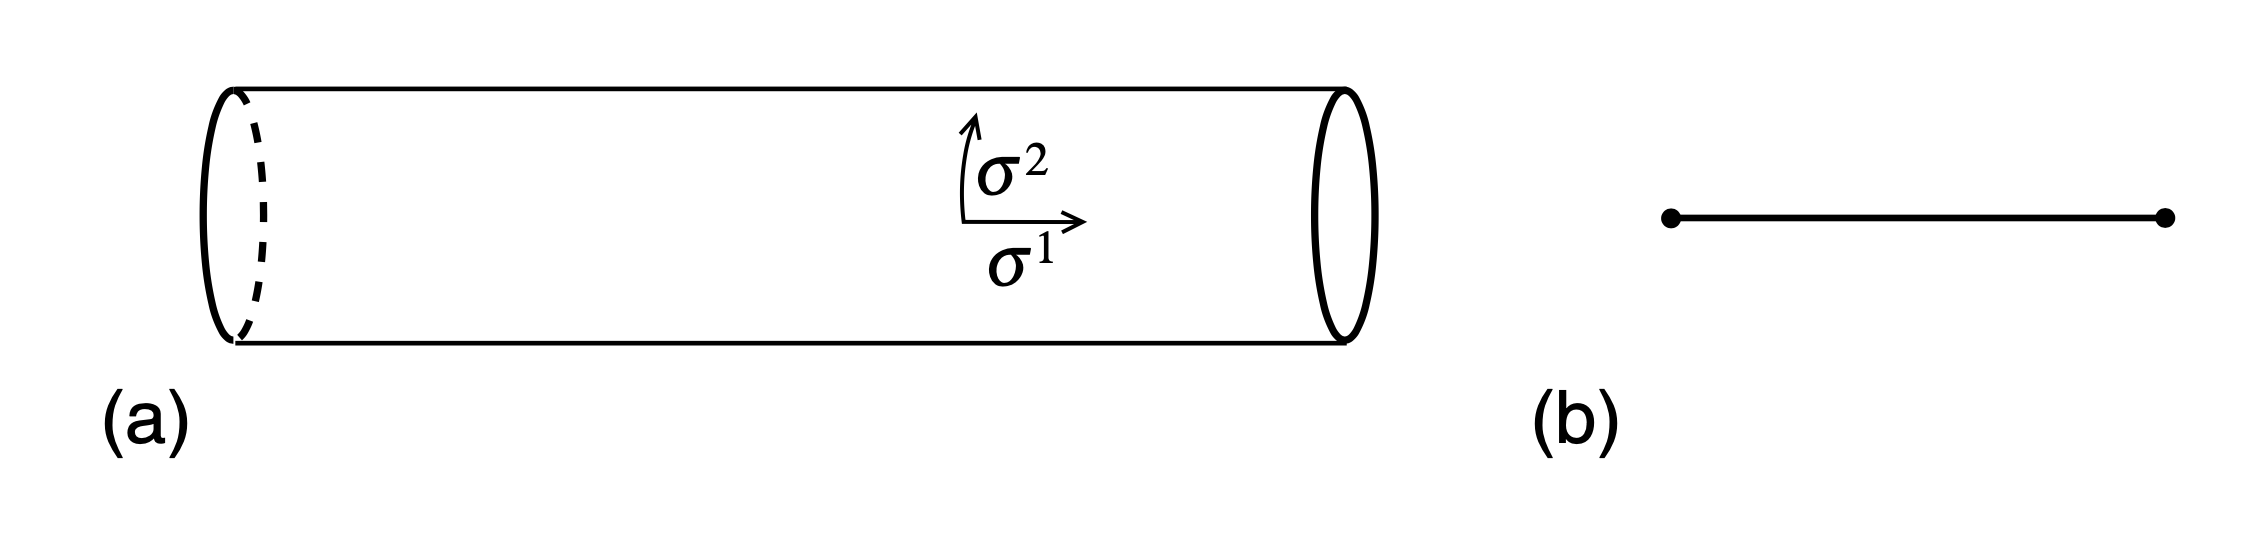
\includegraphics[width=1.0\textwidth]{fig101.png}
    \caption{(a) 小 $t$ 极限下的圆柱. (b) 场论类比图.}
  \end{figure}

首先考察圆柱, 结合玻色弦(\textcolor{red}{7.4.1})在十维中的结果, 再加上费米迹(\ref{10.7.9}), 这里的迹来自\,II\,型弦的一边, 我们把它写成两项的和
\begin{equation}
    Z_{C_{2}}=Z_{C_{2},0}+Z_{C_{2},1} \:, \label{10.8.1}
\end{equation}
其中
\begin{subequations}
    \begin{align}
        Z_{C_{2},0}&=\mi V_{10} n^{2}\int^{\infty}_{0}\frac{\dif t}{8t}(8\pi^{2}\alpha^{\prime}t)^{-5}\eta(\mi t)^{-8}
        \Bigl[Z^{0}{}_{0}(\mi t)^{4}-Z^{1}{}_{0}(\mi t)^{4}\Bigr] \:, \label{10.8.2a} \\
        Z_{C_{2},1}&=\mi V_{10} n^{2}\int^{\infty}_{0}\frac{\dif t}{8t}(8\pi^{2}\alpha^{\prime}t)^{-5}\eta(\mi t)^{-8}
        \Bigl[-Z^{0}{}_{1}(\mi t)^{4}-Z^{1}{}_{1}(\mi t)^{4}\Bigr] \:, \label{10.8.2b}
    \end{align} \label{10.8.2}
\end{subequations}
(注意\,I\,型超弦只能是非定向的, 它来自于\,IIB\,型弦论, 所以$ Z^{1}{}_{1} $前面是负号.) 我们分离这四项是根据迹中是否出现了$ \exp(\pi\mi F)$. $Z_{C_{2},0} $中没有, 所以$ \psi^{\mu} $在$ \sigma_{2} $方向是反周期的. $Z_{C_{2},1} $中有这一项, 所以$ \psi^{\mu} $在$ \sigma_{2} $方向是周期的. 我们也可以认为是圆柱是闭弦从真空中产生又湮灭到真空中. $\psi^{\mu} $的周期性说明$ Z_{C_{2},0} $来自\,NS-NS\,弦而$ Z_{C_{2},1} $来自\,R-R\,闭弦.

由于超对称性, 总的费米弦配分函数为零, 这使得$ Z_{C_{2},1}=-Z_{C_{2},0}$; 我们现在集中考察$ Z_{C_{2},0}$. 利用模变换
\begin{equation}
    \eta_{\mi t} =t^{-1/2} \eta(\mi/t) \:, \qquad Z^{\alpha}{}_{\beta}(\mi t) = Z^{\beta}{}_{-\alpha}(\mi/t)\label{10.8.3}
\end{equation}
定义$ s=\pi/t$, 这变成
\begin{align}
    Z_{C_{2},0} &= \mi \frac{V_{10}n^{2}}{8\pi(8\pi^{2}\alpha^{\prime})^{5}}
    \int \dif s\:\eta(\mi s/\pi)^{-8}\Bigl[Z^{0}{}_{0}(\mi s/\pi)^{4}- Z^{0}{}_{1}(\mi s/\pi)^{4} \Bigr] \nonumber \\
    &=\mi \frac{V_{10}n^{2}}{8\pi(8\pi^{2}\alpha^{\prime})^{5}}
    \int \dif s\: [16 + O(\exp(-2s))] \:. \label{10.8.4}
\end{align}
$s\to\infty $的发散是由于无质量闭弦的蝌蚪图, 注意这必须是\,NS-NS\,态. 我们视其为伸缩子-引力子相互作用 $(-G)^{1/2}\me^{-\Phi}$.

然而这里有一个矛盾: $d=10,N=1 $超对称代数不允许这样的项. 更奇怪的是, $Z_{C_{2},1} $中有一个大小相等, 符号相反的发散, 它只能来自于\,R-R\,态的蝌蚪图, 但是唯一的无质量\,R-R\,态是\,2\,阶张量, 它不可能有\,Lorentz\,不变的蝌蚪图.

可以猜测解决方案是这样的. IIB\,弦对于所有偶数的$ n $有$ n $秩的势, 而$ n $和$ 8-n $在\,Poincar\'{e}\,对偶下相等. $\Omega $投影移去了$ n=0 $和等价的$ n=8$, 以及$ n=4$: 所有\,4\,的倍数. 留下了$,n=2$, 等价的$ n=6 $和$ n=10$. 10\,维中允许存在\,10-form\,势 $C_{10}$, 但是它的\,11-form\,场强$ \dif C_{10} $恒为零. 这个势对时空的积分
\begin{equation}
    \mu_{10}\int C_{10} \label{10.8.5}
\end{equation}
在$ \delta C_{10}=\dif \chi_{9} $下不变, 所以可以出现在作用量中. 由于没有动能项, 这个场的传播子是$ 1/0$, 而蝌蚪图的发散是
\begin{equation}
    \frac{\mu^{2}_{10}}{0} \:. \label{10.8.6}
\end{equation}
这正是$ Z_{C_{2},1} $中发散的起源. 对$ C_{10} $变分给出的运动方程就是$ \mu_{10}=0$, 所以不像之前遇到的发散, 这个发散不能通过背景场的修正移除. 它代表一个真实的不相容性.

\subsection*{The Klein bottle}

还有一种抵消蝌蚪图发散的方法. 圆柱, 莫比乌斯带和克莱因瓶都有来自于无质量闭弦态的发散, 总发散正比于圆盘蝌蚪图与$ RP_{2} $蝌蚪图之和的平方. 两个蝌蚪图的相对大小依赖于\,Chan-Paton\,因子, 对于特定的规范群相互抵消.

为了能对这些贡献求和, 我们必须要重新调整这些曲面, 使得$ \sigma^{2} $方向上的周长和$ \sigma^{1} $方向上的长度一致, 我们分别取其为$ 2\pi $和$ s$. 对于圆柱, 原始的$ \sigma^{1} $的长度为$ \pi $(由于圆柱对应开弦), $\sigma^{2} $方向上的长度为$ 2\pi t$, 所以得到$ s=\pi/t$, 对于克莱因瓶$ s=\pi/2t$, 对于莫比乌斯带$ s=\pi/4t$. 

各个振幅是迹的和, 这些迹来自不同的边界条件和投影. 我们需要通过检验费米子在世界面路径积分上的边界条件决定那些项对\,NS-NS\,交换有贡献, 那些项对\,R-R\,交换有贡献. 在克莱因瓶上, GSO\,投影算符是
\begin{equation}
    \frac{1+\exp(\pi\mi F)}{2} \:,\qquad \frac{1+\exp(\pi\mi\tilde{F})}{2} \:. \label{10.8.7}
\end{equation}
在迹中加入$ R=\Omega \exp(\pi\mi\beta F +\pi\mi\tilde{\beta}\tilde{F})$, 路径积分边界条件是
\begin{subequations}
    \begin{align}
        \psi(w+2\pi\mi t)&= -R\psi(w)R^{-1} =-\exp(\pi\mi\beta)\tilde{\psi}(\bar{w}) \:, \label{10.8.8a} \\
        \tilde{\psi}(\bar{w}+2\pi\mi t)&= -R\tilde{\psi}(\bar{w})R^{-1} =-\exp(\pi\mi\tilde{\beta})\psi(w)\:,\label{10.8.8b}
    \end{align} \label{10.8.8}
\end{subequations}
出现负号是由于费米场. 这给出了
\begin{equation}
    \psi(w+4\pi\mi t) = \exp[\pi\mi(\beta+\tilde{\beta})]\,\psi(w) \:. \label{10.8.9}
\end{equation}
NS-NS\,交换来自在$ \sigma^{2}\to\sigma^{2}+4\pi t $下反对称的截面, 因而来自于计入权重$ \Omega\exp(\pi\mi F)$或$ \Omega\exp(\pi\mi\tilde{F}) $的迹; 更进一步, 这两个迹相等. NS-NS\,态和\,R-R\,态均对这个迹有贡献, 它们各自的贡献是
\begin{subequations}
    \begin{align}
        \text{NS-NS }: \qquad &q^{-1/3}\prod_{m=1}^{\infty} (1+q^{2m-1})^{8} = Z^{0}{}_{0}(2\mi t)^{4} \:, \label{10.8.10a} \\
        \text{R-R }: \qquad &-16 q^{2/3} \prod_{m=1}^{\infty} (1+q^{2m})^{8} =- Z^{1}{}_{0}(2\mi t)^{4} \:,
        \label{10.8.10b}
    \end{align} \label{10.8.10}
\end{subequations}
其中$ q=\exp(-2\pi t)$.

这样, 整个克莱因瓶对\,NS-NS\,交换的贡献就是
\begin{align}
    Z_{K_{2},0} &= \mi V_{10} \int_{0}^{\infty}\frac{\dif t}{8t}\: (4\pi^{2}\alpha^{\prime}t)^{-5} \eta(2\mi t)^{-8}
    \Bigl[ Z^{0}{}_{0}(2\mi t)^{4}-Z^{1}{}_{0}(2\mi t)^{4}\Bigr] \nonumber \\
    &= \mi \frac{2^{10}V_{10}}{8\pi (8\pi^{2}\alpha^{\prime})^{5}}\int^{\infty}_{0}\dif s \: 
    \eta(\mi s/\pi)^{-8} \Bigl[ Z^{0}{}_{0}(\mi s/\pi)^{4}-Z^{1}{}_{0}(\mi s/\pi)^{4} \Bigr] \nonumber \\
    &= \mi \frac{2^{10}V_{10}}{8\pi (8\pi^{2}\alpha^{\prime})^{5}}\int^{\infty}_{0}\dif s \: 
      [16 + O(\exp(-2s))] \:, \label{10.8.11}
\end{align}
并有$ Z_{K_{2},1}=-Z_{K_{2},0}$. 玻色部分与以往相同.


\subsection*{The M\"{o}bius strip}

在开弦上, $\Omega $的作用是
\begin{equation}
    \Omega\psi^{\mu}(w)\Omega^{-1} =\tilde{\psi}(\pi-\bar{w})=\psi^{\mu}(w-\pi) \:,\label{10.8.12}
\end{equation}
这里使用了\,doubing trick (\ref{10.2.15}). 以振子模的形式, 这是
\begin{equation}
    \Omega \psi^{\mu}_{r} \Omega^{-1} =\exp(-\pi\mi r) \,\psi_{r}^{\mu} \:. \label{10.8.13}
\end{equation}
这个相位在\,NS\,截面是虚的且平方等于$ -1$. 因此,
\begin{equation}
    \Omega^{2} =\exp(\pi\mi F) \:. \label{10.8.14}
\end{equation}
根据\,GSO\,投射, $\exp(\pi\mi F)=1$, 在物理上, 它的平方与单位算符相同, 但是$ \Omega $与\,GSO\,的组合投射要求
\begin{equation}
    \frac{1+\Omega +\Omega^{2}+\Omega^{3}}{4} \:. \label{10.8.15}
\end{equation}
现在迹中有$ R=\Omega \exp(\pi\mi\beta F)$, 场的周期性是
\begin{equation}
    \psi^{\mu}(w+4\pi\mi t) = -\exp(\pi\mi\beta)\psi^{\mu}(w+2\pi\mi t-\pi) =\psi^{\mu}(w-2\pi) \:. \label{10.8.16}
\end{equation}
由此得出, 在迹的\,R\,截面中, 场在$ \sigma^{2} $方向上周期的, 对应于\,R-R\,交换, 而迹的\,NS\,截面给出\,NS-NS\,交换.

R-R\,交换要简单一些, 含有$ \Omega $和含有$ \Omega\exp(\pi\mi F) $的迹之和是
\begin{align}
    -16q^{1/3}&\prod_{m=1}^{\infty} [1+(-1)^{m}q^{m}]^{8} 
    -(1-1)^{4}q^{1/3}\prod_{m=1}^{\infty} [1-(-1)^{m}q^{m}]^{8} \nonumber \\
    &= Z^{0}{}_{1}(2\mi t)^{4} Z^{1}{}_{0}(2\mi t)^{4} \:. \label{10.8.17}
\end{align}
整个莫比乌斯振幅是
\begin{align}
    Z_{M_{2},1}&=\pm\mi n V_{10} \int_{0}^{\infty} \frac{\dif t}{8t}(8\pi^{2}\alpha^{\prime}t)^{-5}
    \frac{Z^{0}{}_{1}(2\mi t)^{4}Z^{1}{}_{0}(2\mi t)^{4}}{\eta(2\mi t)^{8}Z^{0}{}_{0}(2\mi t)^{4}}\nonumber \\
    &=\pm 2\mi n \frac{2^{5}V_{10}}{8\pi(8\pi^{2}\alpha^{\prime})^{5}}\int_{0}^{\infty}\dif s \:
    \frac{Z^{0}{}_{1}(2\mi s/\pi)^{4}Z^{1}{}_{0}(2\mi s/\pi)^{4}}{\eta(2\mi s/\pi)^{8}Z^{0}{}_{0}(2\mi s/\pi)^{4}}\nonumber \\
    &=\pm 2\mi n \frac{2^{5}V_{10}}{8\pi(8\pi^{2}\alpha^{\prime})^{5}}\int_{0}^{\infty}\dif s \:
    [16+O(\exp(-2s))] \:, \label{10.8.18}
\end{align}
其中正号对应$ SO(n)$.

R-R\,交换的总发散是
\begin{equation}
    Z_{1} = -\mi(n\mp 32)^{2} \frac{V_{10}}{8\pi (8\pi^{2}\alpha^{\prime})^{5}}
    \int^{\infty}_{0}\dif s \:[16+O(\exp(-2s))] \:. \label{10.8.19}
\end{equation}
R-R\,蝌蚪图对规范群$ SO(32) $为零. 对于每个世界面拓扑, NS-NS\,发散是\,R-R\,发散的负数, 所以伸缩子-引力子蝌蚪对于$ SO(32) $也为零.
